\chapter{INTRODUÇÃO À ESTATÍSTICA}
\section{Contextualização}

Governar a região amazônica é, possivelmente, um dos maiores desafios logísticos e institucionais do planeta. Imagine-se no comando de uma embarcação cruzando o Rio Amazonas em uma noite de neblina intensa. A visibilidade é reduzida, os obstáculos são invisíveis e qualquer decisão precipitada pode comprometer toda a travessia. Administrar políticas públicas em contextos complexos assemelha-se a essa navegação: decisões precisam ser tomadas mesmo sob condições de incerteza. \vskip0.3cm

É nesse cenário que a Estatística assume papel estruturante. Ela não elimina a incerteza, mas a torna mensurável. Não dissipa completamente a neblina, mas fornece instrumentos para estimar riscos, avaliar alternativas e fundamentar escolhas. \vskip0.3cm

Mais do que um conjunto de técnicas quantitativas, a Estatística pode ser compreendida como a infraestrutura cognitiva do Estado moderno. Conforme argumenta \textbf{Hacking (1990)}, o desenvolvimento do pensamento probabilístico alterou profundamente a forma como sociedades passaram a interpretar regularidades coletivas. A noção de acaso deixou de ser mero elemento filosófico para tornar-se categoria operacional na administração de populações. \vskip0.3cm


A Estatística é, na prática, o \textbf{GPS de alta precisão} do gestor público. Ela dissipa a neblina e permite enxergar padrões onde outros veem apenas caos. \vskip0.3cm

Na vasta extensão do Pará, a governança estatal enfrenta questões que não permitem mais o "achismo". Da conservação da \textbf{biodiversidade} à proteção das comunidades indígenas, cada decisão exige base sólida. \vskip0.3cm

\newpage
Quando exploramos os dados de setores-chave como a\textbf{ Bioeconomia} transformando o açaí, o cacau e os óleos essenciais em motores de riqueza sustentável, a estatística nos mostra o caminho para que o lucro não destrua a floresta, mas a mantenha de pé. \vskip0.3cm

Ao analisar indicadores de desenvolvimento humano (educação, renda e saúde), não estamos apenas olhando para planilhas; estamos identificando desigualdades que precisam de correção urgente. Através da análise moderna de dados utilizando desde sensores de satélite que monitoram a floresta em tempo real até algoritmos que preveem safras, é possível formular políticas que equilibrem o crescimento econômico e o bem-estar social.  \vskip0.3cm


Neste contexto, a estatística deixa de ser uma disciplina de cálculos frios para se tornar o ponto de convergência entre a informação bruta e a governança estratégica. \vskip0.3cm

Ela é a linguagem que permite à Amazônia falar com o mundo e, principalmente, com seus próprios gestores, promovendo decisões fundamentadas que garantem a preservação desse patrimônio para as próximas gerações.  \vskip0.3cm


Mas, afinal, o que é \textbf{ESTATÍSTICA}?
\vskip0.3cm

Se você abrir um dicionário antigo, encontrará definições sobre "coleta de dados". Mas para o gestor moderno, a definição é outra: \vskip0.3cm

\begin{center}
\fcolorbox{blue}{white}{Estatística} = \fcolorbox{blue}{white}{é a arte e a ciência de aprender com a incerteza.}
\end{center}

É o conjunto de métodos que nos permite extrair "sinais" úteis de dentro de um "barulho" constante de informações. Se os dados são o novo petróleo da era digital, a estatística é a refinaria que transforma esse recurso bruto em combustível para a tomada de decisão.

\newpage
\section{Etimologia}

O latim é uma língua antiga que teve uma influência significativa no desenvolvimento de várias linguas modernas, e por isso não seria diferente com a palavra estatística, que deriva do latim. 
\vskip0.3cm

Na realidade, pode-se perceber adiante que essa palavra esteve sempre atrelada ao aperfeiçoamento da forma de gerir nações e, mais atualmente, estados-nações. estatística tem raiz na expressão \textbf{Statisticum Collegium}, que significa  (Conselho de Estado). O Conselho de Estado era uma ins\-ti\-tui\-ção específica que existia na Alemanha durante o século XVIII, fundada pelo governo da Baviera. O Statisticum Collegium tinha a finalidade de reunir informações e realizar análises matemáticas relacionadas a assuntos públicos e governamentais. O termo \textbf{Statisticum} foi usado para descrever as atividades e o escopo dessa instituição.\vskip0.3cm

Entretanto, já no final do século XVIII, o termo alemão \textbf{Statistik} foi introduzido pelo primeira vez por Gottfried Achenwall (1749), professor da Universidade de Gottingen, para designar a disciplina matemática que lidava com a coleta, análise e interpretação de dados. 

\vspace{-0.3cm}
\begin{figure}
\centering
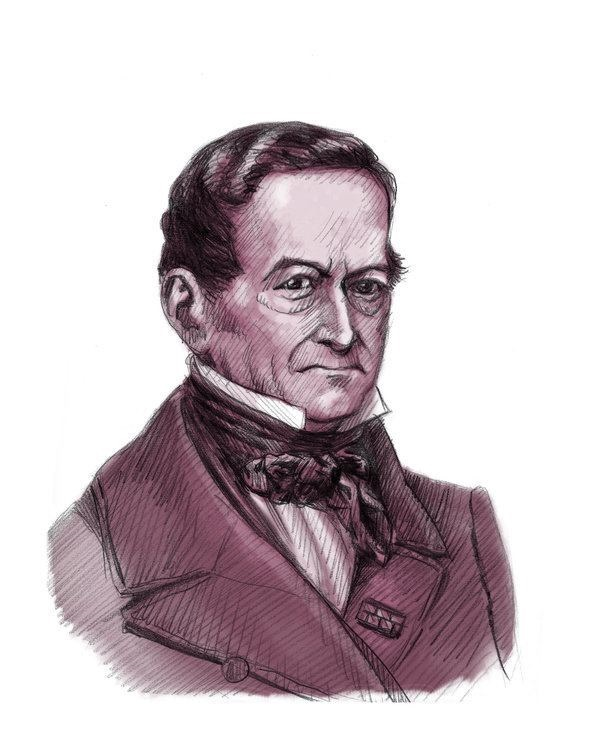
\includegraphics[scale=0.55]{figures/gottfried_achenwall.jpeg}
\vspace{-0.6cm}
\caption{Gottfried Achenwall(1719- 1772)}
\label{fig:my_label8}
\end{figure}


Assim, a palavra Statistik entrou para o vocábulo alemão, influenciada pela evolução e adoção do termo em outros idiomas, como o latim e o italiano. Na Enciclopédia Britânica, o verbete \textbf{Statístics} apareceu em 1797 (STIGLER, 1990).\vskip0.3cm

\newpage
A palavra adquiriu o significado de coleta e classificação de dados em geral através de Sir \textbf{John Sinclair}. Um político, escritor e estatístico britânico do século XVIII e início do século XIX. Desta forma, o propósito original da Statistik era fornecer os dados a serem usados pelo governo e outras organizações. \vskip0.3cm

A coleta de dados sobre estados e localidades continua, em grande parte através de órgãos estatais que cuidam das estatísticas oficiais, realizadas por meio dos Censos. Em particular, os censos fornecem informação regular sobre as populações. De igual modo, a palavra CENSO é derivada do termo latim CENSERE, que significa TAXAR. (STIGLER, 1990).\vskip0.3cm

\section{Aspectos Históricos}
\textbf{"Sem Estatística, Tudo é Uma Mera Opinião."  - W. Edwards Deming} \vskip0.3cm

A estatística surge em conjunto com a organização das sociedades primitivas, que passaram a ter a necessidade do conhecimento numérico de seus recursos disponíveis.  Sendo assim, verifica-se que as primeiras aplicações do pensamento estatístico estavam voltadas para o Estado, fornecendo dados demográficos e econômicos para a criação de políticas públicas, taxação de impostos ou para o (alistamento) serviço militar (EMBRAPA, 2004).\vskip0.3cm

A contagem desempenha papel fundamental na estatística, pois permite que informações quantitativas sejam registradas e representadas de forma numérica. Embora, inicialmente, tenha permanecido em grande parte pouco visível, até porque pouco eram as coisas que precisavam ser contadas pelos povos primitivos, o ato de contar história da Estatística, e o desenvolvimento da matemática e da contabilidade propiciou o desenvolvimento de um método que mais tarde se tornaria Ciência.\vskip0.3cm

Um exemplo notável de registros históricos que evidenciou o nascimento da Estatística remonta a 5000 a.C, quando os antigos egípicios mantinham informações quantitativas sobre prisioneiros de guerra (MEMÓRIA, 2004). Há ainda outros indícios arqueológicos apontando para a falta de mão-de-obra relacionada à construção das pirâmides.\vskip0.3cm

Conforme relato no quarto livro do pentateuco bíblico, no tempo de Moisés, 1400 a.C, Deus ordenara que houvesse a contagem de todos os que poderiam lutar, todos os homens com mais de vinte anos. Um total de 603.550 estavam capacitados para o serviço militar. Ainda dentro do contexto histórico religioso, a narrativa do Evangelho de Lucas aponta que José, junto com a ua esposa Maria, foram de Nazaré até Belém, local onde nasceu Jesus, para serem contados e registrados com fins de tributação e controle administrativo.

\newpage
Este censo foi convocado pelo Imperador romano César Augusto, que havia conquistado aquela região do Oriente Médio (ECHEVESTE et al., 2005). Conforme o Cristianismo se disseminava pelo ocidente, a convicção de que o futuro era moldado por um deus se consolidava entre os povos. Desses registros também se utilizaram as civilizações pré-colombianas dos Maias, Incas e Astecas (LOPES e  MEIRELES, 2005).\vskip0.3cm

Em 1085, Normando Guilherme, "O Conquistador", solicitou um levantamento estatístico da Inglaterra, que deveria conter informações sobre terras, proprietários, uso da terra, empregados e animais, dos conquistados anglo-saxões. Os resultados deste Censo foram publicados em 1086 no livro intitulado "Domesday Book" e serviram de base para o cálculo de impostos. Na Enciclopédia Britânica, o verbete \textbf{STATISTICS} apareceu em 1797. (STIGLER, 1990).\vskip0.3cm

Esses primeiros dados estatísticos representam um marco significativo no desenvolvimento do campo, fornecendo uma base para a análise e compreensão dos eventos sociais e demográficos.

\section{Formação da Estatística no Brasil}

A Educação Estatística tem contribuído muito para o desenvolvimento da sociedade contemporânea, proporcionando instrumentos metodológicos para levantamento de possibilidades, análises de variabilidade, melhoria das previsões e agilidade na tomada de decisões em situação de incerteza (LIMA; GIORDANO; VILHENA, 2023).\vskip0.3cm

No Brasil, a formação da Estatística acompanha a própria construção do Estado e suas necessidades de administração, planejamento e produção de conhecimento sobre o território e a população. Entre os registros históricos, encontram-se solicitações oficiais de envio de informações populacionais e administrativas ao Reino de Portugal ainda no início do século XIX, associadas à necessidade de quantificar recursos e habitantes.\vskip0.3cm

Com a criação de escolas militares e técnicas a partir de 1808, como a Academia Real da Marinha e a Academia Real Militar, consolidou-se um ambiente de ensino de ciências exatas que, progressivamente, abriu espaço para conteúdos ligados à mensuração, ao levantamento de informações e, mais adiante, à Estatística.\vskip0.3cm

Em 1863, a estatística começa a ganhar espaço no campo acadêmico com bases advindas da França, com a criação da cadeira de ``Economia Política, Estatística e Princípios de Direito Administrativo'' na Escola Central, à época lecionada por José Maria Paranhos, futuro Visconde de Rio Branco.\vskip0.3cm

\newpage
Na esfera administrativa, a segunda metade do século XIX marca o fortalecimento de estruturas formais de produção de informação estatal. Em 1872 realizou-se o primeiro Censo Demográfico do Brasil, reconhecido como o primeiro recenseamento geral da população brasileira.

%\footnote{IBGE. \textit{Histórico dos censos}. Memória IBGE. Disponível em: \url{https://memoria.ibge.gov.br/historia-do-ibge/historico-dos-censos}. Acesso em: 06 maio 2026.} 

\vskip0.3cm

Em 1934, foi criada a Faculdade de Filosofia, Ciências e Letras - FFCL da Universidade de São Paulo - USP, consolidando a cadeira de Estatística Geral e Aplicada em cursos como Ciências Sociais e Pedagogia (PEREIRA; MORETTIN, 1991).\vskip0.3cm

No século XX, a institucionalização se fortalece com a criação do Instituto Nacional de Estatística (INE) em 1934 e sua instalação em 1936; em 1938, o órgão passa a denominar-se Instituto Brasileiro de Geografia e Estatística (IBGE), consolidando-se como referência nacional para produção de estatísticas oficiais e informações geocientíficas.

%\footnote{IBGE. \textit{Linha do tempo do IBGE}. Memória IBGE. Disponível em: \url{https://memoria.ibge.gov.br/images/memoria/documentos/linha-do-tempo-IBGE.pdf}. Acesso em: 06 maio 2026.} 

\vskip0.3cm

Em meados de 1946, a FFCL/USP regulamentou iniciativas pioneiras de pós-graduação em Estatística no Brasil (LOPES, 1988).\vskip0.3cm

Em 1953, destaca-se a criação da Escola Nacional de Ciências Estatísticas (ENCE), vinculada ao IBGE, voltada à formação especializada de quadros técnicos para o sistema estatístico nacional.

%\footnote{ENCE/IBGE. \textit{70 anos da ENCE: uma breve história}. Disponível em: \url{https://ence.ibge.gov.br/noticias/2506-70-anos-da-ence-uma-breve-historia.html}. Acesso em: 06 maio 2026.} 

\vskip0.3cm

A partir da década de 1970, a difusão da computação e a ampliação do uso de métodos quantitativos nas políticas públicas e nas ciências aplicadas impulsionaram a produção estatística e a demanda por formação em Estatística nas universidades. Mais recentemente, a consolidação de infraestruturas de dados, a cultura de dados abertos e o avanço de metodologias computacionais (por exemplo, ciência de dados e aprendizado de máquina) intensificaram o papel da Estatística no planejamento governamental e na pesquisa.\vskip0.3cm

Um exemplo contemporâneo da centralidade dessas informações é o Censo Demográfico de 2022, conduzido pelo IBGE, cujos resultados vêm subsidiando políticas públicas, fundos de participação, planejamento urbano e análises socioeconômicas em todo o país.

%\footnote{IBGE. \textit{Censo 2022}. Disponível em: \url{https://censo2022.ibge.gov.br/}. Acesso em: 06 maio 2026.} 

\vskip0.3cm

Na educação escolar, esse movimento chega com maior força em 1997, com a publicação dos PCN (Parâmetros Curriculares Nacionais), que incorporam oficialmente o ``Tratamento da Informação'' como bloco de conteúdos de Matemática na Educação Básica (BRASIL, 1997; VILAS BÔAS; KONTI, 2018).\vskip0.3cm

Com os PCN, o ensino brasileiro de Estatística amplia seu campo de investigação e passa a demandar produção acadêmica alinhada às novas exigências curriculares (SANTOS, 2015). 

\newpage
Para Samá (2019), a inclusão formal de Estatística e Probabilidade na Educação Básica impulsionou pesquisas em Educação Estatística, especialmente no que se refere à inserção desses conceitos na escola e à formação docente, historicamente insuficiente para dar conta dessa agenda.\vskip0.3cm

A fim de integrar os pesquisadores interessados na área, em 2000, é criado o grupo de trabalho em Ensino de Estatística e Probabilidade - GT12, durante o primeiro Seminário Internacional de Pesquisa em Educação Matemática (SIPEM), promovido pela Sociedade Brasileira de Educação Matemática (SBEM). Este GT foi concebido no intuito de estudar os processos referentes ao ensino e à aprendizagem de Estatística, o que, segundo ementa do GT12, envolve aspectos cognitivos e afetivos, além da epistemologia dos conceitos estatísticos e o desenvolvimento de estratégias didáticas com vistas a desenvolver o letramento estatístico. \vskip0.3cm

De acordo com Vilas Bôas e Konti (2018), nos últimos anos, muitos educadores matemáticos e estatísticos têm dedicado grandes segmentos de suas carreiras para aprimorar os materiais e técnicas pedagógicas para a educação estatística. Esse movimento pode ser considerado como base para o que se denomina atualmente de Educação Estatística. \vskip0.3cm

Hoje podemos dizer que a Educação Estatística, enquanto área de pesquisa, objetiva estudar e compreender a forma como as pessoas ensinam e aprendem estatística, englobando a epistemologia dos conceitos estatísticos, os aspectos cognitivos e afetivos do ensino e da aprendizagem, bem como o desenvolvimento de metodologias e materiais para o ensino. \vskip0.3cm

Em 2018, a Base Nacional Comum Curricular(BNCC) consolida a unidade temática Probabilidade e Estatística, com caráter normativo, orientando o desenvolvimento de habilidades de coleta, organização, representação, interpretação e análise de dados ao longo da Educação Básica (BRASIL, 2018).\vskip0.3cm


\newpage
\subsection{Panorama Atual: Cursos de Estatística no Brasil}
\vskip0.2cm

A Tabela~\ref{tab:cursos-estatistica-brasil} apresenta um quadro para organizar, em nível nacional, instituições que oferecem curso de Estatística no Brasil. \vskip0.2cm



{\small
\setlength{\tabcolsep}{3pt}
\renewcommand{\arraystretch}{1.05}
\begin{longtable}{p{5.2cm}p{1.2cm}p{0.8cm}p{2.6cm}p{2.6cm}}
\caption{Instituições com oferta de curso de Estatística no Brasil (levantamento a partir de conselhos profissionais e p\'aginas institucionais; conferir atualiza\c{c}\~oes).}\label{tab:cursos-estatistica-brasil}\\
\toprule
\textbf{INSTITUIÇÃO} & \textbf{SIGLA} & \textbf{UF} & \textbf{CIDADE} & \textbf{TURNO}\\
\midrule
\endfirsthead

\toprule
\textbf{Instituição} & \textbf{Sigla} & \textbf{UF} & \textbf{Cidade} & \textbf{Turno}\\
\midrule
\endhead

\midrule
\multicolumn{5}{r}{\textit{Continua...}}\\
\endfoot

\bottomrule
\endlastfoot

Universidade Federal do Par\'a & UFPA & PA & Bel\'em & Vespertino\\
Universidade Federal do Amazonas & UFAM & AM & Manaus & Diurno\\
Universidade Federal de Rond\^onia & UNIR & RO & Ji-Paran\'a & Noturno\\
Universidade Federal do Cear\'a & UFC & CE & Fortaleza & Diurno\\
Universidade Estadual da Para\'iba & UEPB & PB & Campina Grande & Matutino\\
Universidade Federal de Campina Grande & UFCG & PB & Campina Grande & Diurno\\
Universidade Federal da Para\'iba & UFPB & PB & Jo\~ao Pessoa & Matutino\\
Universidade Federal do Rio Grande do Norte & UFRN & RN & Natal & Matutino\\
Universidade Federal de Pernambuco & UFPE & PE & Recife & Diurno\\
Universidade Federal da Bahia & UFBA & BA & Salvador & Diurno\\
Universidade Federal de Sergipe & UFS & SE & S\~ao Crist\'ov\~ao & Noturno\\
Universidade Federal do Piau\'i & UFPI & PI & Teresina & Noturno\\
Universidade de Bras\'ilia & UnB & DF & Bras\'ilia & Diurno\\
Universidade Federal de Goi\'as & UFG & GO & Goi\^ania & Noturno\\
Universidade Federal de Mato Grosso & UFMT & MT & Cuiab\'a & Noturno\\
Universidade Federal de Minas Gerais & UFMG & MG & Belo Horizonte & Diurno\\
Universidade Federal de Juiz de Fora & UFJF & MG & Juiz de Fora & Diurno\\
Universidade Federal de Ouro Preto & UFOP & MG & Ouro Preto & Noturno\\
Universidade Federal de Uberl\^andia & UFU & MG & Uberl\^andia & Noturno\\
Universidade Federal de Lavras & UFLA & MG & Lavras & Diurno\\
Universidade Federal Fluminense & UFF & RJ & Niter\'oi & Integral\\
Escola Nacional de Ci\^encias Estat\'isticas (IBGE) & ENCE & RJ & Rio de Janeiro & Diurno\\
Universidade do Estado do Rio de Janeiro & UERJ & RJ & Rio de Janeiro & Diurno\\
Universidade Federal do Rio de Janeiro & UFRJ & RJ & Rio de Janeiro & Diurno\\
Universidade Estadual Paulista (campus Presidente Prudente) & UNESP & SP & Presidente Prudente & Diurno\\
Universidade Estadual de Campinas & UNICAMP & SP & Campinas & Diurno\\
Universidade Federal de S\~ao Carlos & UFSCar & SP & S\~ao Carlos & Diurno\\
Universidade de S\~ao Paulo (campus S\~ao Carlos) & USP & SP & S\~ao Carlos & Noturno\\
Universidade de S\~ao Paulo (campus S\~ao Paulo) & USP & SP & S\~ao Paulo & Diurno\\
Faculdades Metropolitanas Unidas & FMU & SP & S\~ao Paulo & Noturno\\
Universidade Federal do Esp\'irito Santo & UFES & ES & Vit\'oria & Diurno\\
Universidade Federal do Paran\'a & UFPR & PR & Curitiba & Noturno\\
Universidade Estadual de Maring\'a & UEM & PR & Maring\'a & Noturno\\
Universidade Federal do Rio Grande do Sul & UFRGS & RS & Porto Alegre & Diurno\\
Universidade Federal de Santa Maria & UFSM & RS & Santa Maria & Noturno\\
\end{longtable}
{\footnotesize\textit{Fonte}: CONRE-3/2026.}\vskip0.3cm
}

Dessa forma, constitui-se em um grande avanço para o ensino de Estatística no Ensino Fundamental. Em suas diretrizes há a intenção do desenvolvimento de competências para o pensamento e raciocínio estatístico, contribuindo, certamente, para a formação de cidadãos mais conscientes sobre as informações que circulam no meio educacional e no mundo. Estas perspectivas apontam que as pessoas saibam tomar decisões, diante de questões políticas e sociais, pois delas também dependem da leitura e interpretação de informações complexas, muitas vezes contraditórias.\vskip0.3cm


\newpage
Nesse desenvolvimento, o estudo de algumas noções ganha espaço no ensino nos anos iniciais, como: tabelas, gráficos, quadros, pesquisa etc. e a noção de chance (mais provável, pouco provável, acontecerá com certeza, talvez aconteça, é impossível de acontecer etc.) ligadas à introdução de ideias de probabilidade. “Contudo, os professores que lecionam Matemática nos anos iniciais confessam que, quando estudaram Estatísticas e Probabilidade, nos cursos de Pedagogia ou em Matemática, não viram esses conteúdos como objetos a serem ensinados na escola básica, especialmente para alunos da educação infantil e anos iniciais” (LOPES, 2008). \vskip0.3cm

Assim, os professores em exercício, em grande parte, não tiveram formação adequada para tratar o assunto e, na formação continuada, se apropriam de métodos de como proceder para lecionar sem se aprofundar nos conhecimentos de base para terem domínio que os possibilitem criarem e não só compilarem tarefas (LIMA et al., 2023). \vskip0.3cm

Diante disso, para que o cidadão sobreviva e assimile este mar de estatística, é necessário que alguns conceitos sejam trabalhados desde a escola.

\section{Conceitos Fundamentais em Estatística}
\subsection{O Que é Ciência Estatística}

Definir a Estatística é um desafio devido à sua vasta aplicabilidade, mas podemos compreendê-la como a ponte entre o caos dos dados e a clareza da decisão. Segundo Rao (1973), ela pode ser resumida em uma equação elegante: 

\begin{center}
\fcolorbox{blue}{white}{ Conhecimento Incerto} + \fcolorbox{blue}{white}{Incerteza}  = \fcolorbox{blue}{white}{Conhecimento Útil} 
\end{center}

Na gestão pública, isso significa que o objetivo da Estatística é analisar dados que, embora sujeitos a variações e imprevistos, fornecem o subsídio necessário para o planejamento e a obtenção de resultados concretos para a sociedade (RAO, 1999). É a ciência que transforma a dúvida em direção estratégica. \vskip0.3cm

Diferentes autores reforçam essa visão multidimensional. Enquanto Stein \& Loesch (2008) a definem como a ciência da coleta, organização e análise de dados amostrais, o Dicionário Aurélio (2005) destaca seu papel em fazer predições. Já Motta \& Wagner (2003) e Cazorla et al. (2017) enfatizam que a Estatística é uma ciência metodológica fundamental que permite interpretar fenômenos por meio de variáveis numéricas. \vskip0.3cm

Em suma, ela não é apenas um conjunto de fórmulas, mas uma ferramenta para o desenvolvimento da autonomia e do juízo crítico do gestor (LOPES, 2010), permitindo que ele aprenda com os dados e valide hipóteses sobre a realidade social. \vskip0.3cm

\subsection{Estatística vs. Matemática}

Embora caminhem juntas, a Estatística é uma ciência distinta da Matemática. Como aponta Matsushita (2010), seus objetos de estudo são diferenciados: a Estatística lida com o mundo real e suas imperfeições. Para Cobb e Moore (1997), a grande força da Estatística está em saber lidar com a variabilidade. Enquanto a Matemática pode lidar com números abstratos, na Estatística os números são "números com contexto".  \vskip0.3cm

Um dado não se interpreta sozinho; como bem afirma Moore (2000), ele deve ser lido com entendimento, tal qual as palavras em um argumento. Para o gestor, isso significa que um índice de desmatamento ou uma taxa de mortalidade não são apenas algarismos, mas histórias que exigem leitura crítica e interpretação fundamentada. \vskip0.3cm

Nesse contexto, o pensamento estatístico pode ser definido como a capacidade de utilizar e/ou interpretar, de forma adequada, as ferramentas estatísticas na solução problemas. Isto envolve o entendimento da essência dos dados e da possibilidade de fazer inferências, assim como o reconhecimento e a compreensão do valor da Estatística como uma disposição para pensar numa perspectiva da incerteza (CAZORLA et al, 2017). \vskip0.3cm

Assim, é possível distinguir duas concepções para a palavra ESTATÍSTICA: no plural (estatísticas), indica qualquer coleção de dados numéricos, reunidos com a finalidade de fornecer informações acerca de uma atividade qualquer. Assim, por exemplo, as estatísticas demográficas referem-se aos dados numéricos sobre nascimentos, falecimentos, matrimônios, desquites, etc. As estatísticas econômicas consistem em dados numéricos relacionados com emprego, produção, vendas e com outras atividades ligadas aos vários setores da vida econômica. \vskip0.3cm

No singular (Estatística), indica a atividade humana especializada ou um corpo de técnicas, ou ainda uma metodologia desenvolvida para a coleta, a classificação, a apresentação, a análise e a interpretação de dados quantitativos e a utilização desses dados para a tomada de decisões.\vskip0.3cm

O mundo está repleto de problemas. Para resolver a maioria deles, necessitamos de informações. Mas, que tipo de informação? Que quantidade de informações? Após obtê-las, o que fazer com elas? A Estatística trabalha com essas informações, associando ao problema, descobrindo como e o que coletar de dados, assim capacitando o pesquisador a obter conclusões a partir dessas informações, de tal forma que possam ser entendidas por outras pessoas. \vskip0.3cm


Portanto, os métodos estatísticos auxiliam o cientista social, o economista, o engenheiro, o biólogo, o agrônomo e muitos outros profissionais a realizarem o seu trabalho com mais eficiência.\vskip0.3cm

Assim, uma igualdade que pode sintetizar as considerações descritas anteriormente sobre a estatística pode ser expressa como (PADOVANI, 2012):

\begin{center}
\fcolorbox{blue}{white}{ESTATÍSTICA} = \fcolorbox{blue}{white}{CIÊNCIA} + \fcolorbox{blue}{white}{TECNOLOGIA} + \fcolorbox{blue}{white}{ARTE}
\end{center}

A Estatística se divide didaticamente em duas partes: Descritiva e Inferencial


\subsection{Estatística Descritiva, Dedutiva, Analítica ou Numérica}

Muitas vezes, o gestor público lida com um volume tão massivo de informações que se torna impossível compreendê-las intuitivamente. É aqui que entra a Estatística Descritiva. Seu objetivo, conforme Toledo e Ovalle (1995) e Stein e Loesch (2008), é descrever, resumir e sumariar um conjunto de dados para que a informação se torne concisa e compreensível. \vskip0.3cm

Através de métodos gráficos, tabulares e numéricos, ela transforma planilhas intermináveis em indicadores claros. Além de sintetizar o presente, a análise descritiva é essencial para identificar anomalias ou erros de registro, garantindo que a base da decisão seja confiável e livre de "estatísticas obscuras" que possam distorcer a realidade (CAMEY et al., 2010).

\subsection{Estatística Indutiva, Amostral ou Inferencial}

Na prática governamental, observar toda uma população é frequentemente impossível devido aos altos custos e dificuldades operacionais. A solução é a Estatística Inferencial. Ela permite que o pesquisador examine uma parte representativa (a amostra) e, com base nela, tire conclusões válidas para todo o grupo (CASTANHEIRA, 2005).  \vskip0.3cm

Imagine testar a qualidade da água em um porto ou a eficácia de um novo medicamento: não examinamos cada gota ou cada paciente, mas generalizamos os resultados da amostra com um grau calculado de confiança. Esse processo lida diretamente com a incerteza e utiliza a Teoria das Probabilidades para garantir que as afirmações sobre a população tenham fundamentação científica e segurança técnica. 


A estatística inferencial pode ser classificada em:

\begin{enumerate}
  \item \textbf{Estimação de Parâmetros}: inferências sobre os parâmetros (descritores matemáticos como média, desvio-padrão, proporções, risco relativo, correlação, etc.) na população em estudo baseada em estatísticas análogas (estimadores dos parâmetros) obtidos a partir da amostra.
  \item \textbf{Teste de Significância}: as probabilidades são calculadas com base em hi\-pó\-te\-ses sobre a associação exposição-desfecho na população em estudo.
\end{enumerate}

\subsection{Fenômeno + Experimento + Dado Estatístico}

Tudo o que o gestor pretende analisar, seja o fluxo de pessoas em um hospital ou a produtividade agrícola, é um fenômeno estatístico. Esses fenômenos podem ser coletivos (massa), individuais ou de multidão, onde o comportamento do grupo difere do particular. \vskip0.3cm

Para estudar esses eventos, utilizamos o experimento aleatório, que produz resultados variados mesmo sob condições idênticas, devido ao acaso. O resultado dessas observações é o dado estatístico, a matéria-prima que descreve a realidade. \vskip0.3cm

Hoje, esses dados são organizados em Matrizes de Dados (planilhas), onde cada linha representa uma unidade observacional (um cidadão, uma escola) e cada coluna representa uma variável, a característica específica que estamos medindo e que varia entre cada indivíduo.


\subsection{História Estatística com Dados}

Grande parte da visualização de dados tem como finalidade a comunicação. Quando analisamos um conjunto de informações, buscamos compartilhar nossa interpretação com um público específico. Para que essa mensagem seja eficaz, não basta apenas apresentar números: é necessário organizá-los em uma história clara, coerente e envolvente.. \vskip0.3cm

Muitas vezes, a ideia de “contar histórias” pode soar estranha para cientistas, jornalistas ou gestores públicos, que associam o termo a invenção ou exagero. Contudo, a narrativa não deve ser entendida como manipulação, mas sim como uma estratégia de tradução: ela conecta números a contextos reais, favorecendo a compreensão e a memória coletiva (UNECE, 2009). \vskip0.3cm

Os especialistas em estatística geralmente dominam a técnica de representar dados de forma correta, mas nem sempre se preocupam com a estética visual ou com a clareza narrativa. Por outro lado, profissionais de design podem produzir gráficos atraentes, mas com pouca fidelidade metodológica. O desafio está em conciliar precisão técnica com comunicação acessível, de modo que a estatística cumpra seu papel social.

%(WILKE, 2019). 
\subsubsection{O Que é uma História Estatística}

Estatísticas, isoladamente, são apenas números que circulam em diferentes esferas da vida cotidiana: resultados esportivos, indicadores econômicos, variações de mercado, entre outros. No entanto, o verdadeiro valor da estatística não está no número bruto, mas na capacidade de revelar padrões, tendências e implicações sociais.


\newpage
Uma história estatística pode ser definida como uma narrativa que organiza fatos e evidências de forma sequencial, despertando interesse e produzindo significado para o público. Ela vai além da simples exposição de tabelas e gráficos, respondendo perguntas essenciais:

\begin{itemize}
    \item Quem está envolvido?
    \item Quando e onde os eventos ocorreram?
    \item Quais são as causas e consequências?
\end{itemize}

Ao integrar essas dimensões, os dados tornam-se mais compreensíveis e memoráveis. Em vez de recordar cifras exatas, o público se conecta com a mensagem central transmitida pelos números. É essa abordagem que transforma estatísticas em instrumentos de decisão e mudança social. \vskip0.3cm 

Uma História Estatística pode:

\begin{itemize}
    \item Fornecer conhecimento geral, algumas perspectivas, e um certo contexto;
    \item Informar o debate sobre algumas questões específicas.
\end{itemize}

Em termos jornalísticos, o número por si só não é a história. Uma história estatística mostra aos leitores o significado, a importância e a relevância das informações mais atuais. Em outras palavras, responde à pergunta: por que meu público deveria querer ler sobre isso?\vskip0.3cm 

Finalmente, uma história estatística deve conter material digno de nota. Pergunte a si mesmo: a informação é suficientemente importante e inovadora para atrair a cobertura da mídia? A mídia pode escolher um foco diferente. Mas ela tem muitos outros fatores a considerar ao escolher um enredo.

Contar histórias estatísticas é sobre:

\begin{itemize}
    \item Chamar a atenção do leitor com um título ou imagem;
    \item Fornecer a história por trás dos números de forma fácil de entender, interessante e divertida;
    \item Encorajar leitores e outros a considerar como as estatísticas podem adicionar impacto a quase todas as histórias que eles têm para contar.
\end{itemize}

\subsubsection{Por Que Contar uma História Estatística}

Há dois motivos principais para que órgãos públicos e institutos de pesquisa invistam em narrativas estatísticas:

\begin{enumerate}
    \item Cumprimento de sua missão institucional: agências estatísticas têm o dever de informar a sociedade sobre sua realidade demográfica, social, econômica e cultural, permitindo que cidadãos tomem decisões mais conscientes.
    \item Fortalecimento da relevância pública: quando os dados são apresentados de forma clara e contextualizada, aumentam a confiança da população, a colaboração de respondentes e a legitimidade das políticas baseadas em evidências.
\end{enumerate}

Na prática, as estatísticas são difundidas principalmente pela internet e pela mídia tradicional. A primeira facilita o acesso direto aos bancos de dados oficiais, enquanto a segunda continua sendo o principal meio de popularização da informação. Em ambos os casos, a narrativa estatística deve ser precisa, transparente e acessível, sem jamais comprometer a confidencialidade dos dados individuais.


\subsubsection{Fluxo de Trabalho para Contar Histórias com Dados}

Para estruturar uma boa história estatística, é útil adotar um fluxo de trabalho em cinco etapas:

\begin{itemize}
\item[{a)}] \textbf{Planejar e definir o objetivo final}: estabelecer a mensagem central que se pretende comunicar.
\item[{b)}] \textbf{Simular e avaliar cenários}: antecipar possíveis formatos de dados e padrões esperados.
\item[{c)}] \textbf{Coletar e preparar os dados reais}: etapa crítica que envolve organização, padronização e limpeza.
\item[{d)}] \textbf{Explorar e compreender os dados}: aplicação de estatísticas descritivas, testes de hipóteses e modelos explicativos.
\item[{e)}] \textbf{Comunicar os resultados}: traduzir achados em uma narrativa clara, acompanhada de visualizações adequadas.
\end{itemize}

Esse processo deve sempre respeitar cinco princípios fundamentais:

\begin{itemize}
\item \textbf{Comunicação eficaz};
\item \textbf{Reprodutibilidade das análises};
\item \textbf{Ètica e transparência};
\item \textbf{Precisão Metodológica};
\item \textbf{Proteção à confiabilidade dos dados}.
\end{itemize}


\newpage
\subsection{História Estatística versus Storytelling}

A ideia de construir uma \textit{história estatística} com dados emerge da necessidade de transformar informações numéricas em narrativas compreensíveis e socialmente relevantes. Esse conceito está intimamente ligado ao \textit{storytelling}, uma prática milenar de comunicação que se baseia em personagens, enredos e emoções para transmitir valores, ensinamentos ou persuadir públicos específicos. Ao transpor essa lógica para o campo da estatística, o pesquisador passa a desempenhar um papel não apenas técnico, mas também pedagógico e comunicativo: traduzir indicadores e resultados em mensagens que façam sentido para gestores, cidadãos e instituições públicas.\vskip0.3cm

Enquanto o \textit{storytelling} tradicional utiliza recursos simbólicos e ficcionais para engajar a audiência, a história estatística estrutura-se sobre evidências concretas, geralmente extraídas de registros oficiais, censos, inquéritos e sistemas de monitoramento. Os números passam a desempenhar, nesse caso, o papel de personagens principais, carregando consigo a responsabilidade de representar realidades coletivas. 

Um gráfico de evolução da taxa de mortalidade infantil, por exemplo, não é apenas uma curva em um eixo cartesiano: ele representa vidas, políticas públicas e a eficácia (ou ausência) de ações estatais ao longo do tempo.\vskip0.3cm

No campo da gestão pública, essa perspectiva adquire relevância estratégica. O gestor que acessa relatórios frios, compostos apenas por tabelas e séries históricas, pode encontrar dificuldades em interpretar padrões, estabelecer prioridades ou justificar decisões. Entretanto, quando os mesmos dados são apresentados dentro de uma narrativa estatística — contextualizados com causas, consequências e comparações regionais — tornam-se insumos poderosos para o planejamento e a formulação de políticas públicas. Assim, a estatística deixa de ser vista como uma disciplina abstrata, restrita a cálculos técnicos, e passa a ser reconhecida como uma linguagem que conecta o Estado à sociedade.\vskip0.3cm

No caso do Estado do Pará, essa abordagem pode ser ilustrada em diferentes áreas. Ao relatar o crescimento da frota veicular nos municípios paraenses, por exemplo, não basta indicar que o número de veículos aumentou 45\% em dez anos. É necessário narrar o impacto desse crescimento sobre a mobilidade urbana, a necessidade de expansão da infraestrutura viária e os desafios de segurança no trânsito. Da mesma forma, a análise estatística da taxa de escolarização não se resume a percentuais: ela pode contar uma história sobre inclusão social, investimento em educação básica e desigualdades regionais entre o interior e a capital. Em ambos os casos, a narrativa construída a partir dos números revela problemas, aponta conquistas e sugere caminhos para o futuro.\vskip0.3cm

\newpage
Outro aspecto central dessa conexão entre estatística e storytelling está na dimensão ética. Uma narrativa baseada em dados deve prezar pela fidelidade metodológica, pela transparência nas fontes e pela reprodutibilidade dos cálculos. Diferentemente de histórias tradicionais, que podem recorrer à imaginação e ao simbolismo, a história estatística precisa manter compromisso com a veracidade e com o interesse público. Nesse sentido, o uso inadequado ou manipulativo dos números compromete não apenas a qualidade da informação, mas também a confiança da sociedade nas instituições estatais.\vskip0.3cm

Portanto, a história estatística com dados não substitui o \textit{storytelling} tradicional, mas dialoga com ele, incorporando sua lógica de comunicação para potencializar a compreensão dos fenômenos sociais. Ambos compartilham o mesmo objetivo central: dar sentido às informações e aproximá-las do público. Se o \textit{storytelling} aproxima as pessoas de experiências humanas por meio da emoção, a história estatística aproxima os cidadãos da realidade social por meio da evidência. Ao final, o que se busca é uma narrativa que não apenas informe, mas que engaje, inspire e possibilite transformações concretas no espaço público.


%Nas últimas décadas, a discussão sobre comunicação estatística ganhou centralidade com o avanço da ciência de dados e da transparência pública. Tufte (2001) enfatiza que a apresentação gráfica deve preservar integridade quantitativa, evitando distorções visuais que comprometam a interpretação. De modo complementar, Wilke (2019) argumenta que a clareza visual constitui parte essencial da responsabilidade científica. No contexto da gestão pública, comunicar resultados com precisão e honestidade é tão relevante quanto produzi-los. \vskip0.3cm

\newpage
Nesse contexto, a Tabela 1.1, apresentada a seguir, sintetiza as principais diferenças e convergências entre a narrativa estatística e o storytelling tradicional, destacando o papel de cada um na construção de mensagens eficazes para diferentes públicos.


\begin{table}[H]
\centering
\caption{Comparação entre História Estatística com Dados e Storytelling Tradicional}
\label{tab:historia_vs_storytelling}
\begin{tabular}{|p{3.5cm}|p{4.2cm}|p{4.2cm}|}
\hline
\textbf{Aspecto} & \textbf{História Estatística com Dados} & \textbf{Storytelling Tradicional} \\ \hline
\textbf{Base} & Evidências numéricas, indicadores e registros oficiais & Experiências, ficção, metáforas ou relatos pessoais \\ \hline
\textbf{Objetivo} & Traduzir dados em mensagens claras, úteis e verificáveis para orientar decisões & Envolver, entreter ou inspirar pela emoção e pelo enredo \\ \hline
\textbf{Linguagem} & Técnica, mas acessível; busca clareza e precisão sem perder o engajamento & Narrativa livre, com foco em personagens, conflito e clímax \\ \hline
\textbf{Rigor} & Exige reprodutibilidade, ética e fidelidade aos dados & Pode ser subjetivo, simbólico e até ficcional \\ \hline
\textbf{Aplicações} & Gestão pública, relatórios estatísticos, divulgação científica, jornalismo de dados & Literatura, cinema, marketing, discursos, comunicação interpessoal \\ \hline
\textbf{Exemplo} & Relatório sobre taxa de desemprego no Pará, contextualizando causas e efeitos & Filme que conta a trajetória de superação de um personagem \\ \hline
\end{tabular}
\begin{flushleft}
\footnotesize \textbf{Fonte}: KNAFLIC (2018).
\end{flushleft}
\end{table}

%KNAFLIC, Cole Nussbaumer. Storytelling com dados: um guia de visualização de dados para profissionais de negócios. Tradução de João Tortello. Rio de Janeiro: Alta Books, 2018.


\newpage
\subsection{Estatísticas Vitais}

As estatísticas vitais se baseiam em dados coletados de registros de eventos vitais, como nascimento e mortes. Assim, na área de saúde os profissionais precisam ser capazes de interpretar  estatísticas vitais a fim de diagnosticar e tratar pacientes de modo eficaz.

\subsection{Hipótese Estatística}

Em termos simples, uma \textbf{hipótese} é uma resposta possível de ser testada e fundamentada para uma pergunta feita relativa ao fenômeno escolhido. O pesquisador examina a literatura sobre ao fenômeno, obtêm a maior quantidade de conhecimento possível para responder ao problema formulado. Esta tentativa de resposta é a hipótese (HIRAKATA et al, 2019).\vskip0.3cm    

As hipóteses podem ser formuladas dependendo do tipo de problema, de três maneiras

\begin{enumerate}
\item \textbf{Hipóteses Univariadas}: são os que apresentam uma variável;  
\item \textbf{Hipóteses Multivariadas}: são os que apresentam ligação entre duas va\-ri\-á\-veis;
\item \textbf{Hipóteses de Relação Casual}: são os que apresentam Relação de causa e efeito entre as variáveis.
\end{enumerate}

Existem algumas exigências para formulação de hipóteses:

\begin{itemize}
\item formular hipóteses clara e precisas. Convêm estabelecer tanto as hipóteses de pesquisa, quanto as de nulidade.  
\item indicar a importância e contribuição teórica das hipóteses.
\item definir as variáveis, preferencialmente em termos operacionais, distinguindo as variáveis independentes e dependentes. 
\end{itemize}

Para Hirakata (et al, 2019) a hipótese estatística é uma suposição formulada a respeito dos parâmetros de uma ou mais populações e é testada a partir dos resultados amostrais. 

\subsubsection{Teste de Hipóteses}

O teste de hipóteses é um método de averiguação sobre a veracidade de uma afirmação, associado a um risco máximo de erro. Em termos estatísticos, um teste de hipóteses é uma regra de decisão para aceitar ou rejeitar uma hipótese, com base nas informações fornecidas pelos dados coletados em uma amostra (CALLEGARI-JACQUES, 2013).\vskip0.3cm

%Soares JF, Siqueira AL. Introdução à estatística médica. Belo Horizonte: Coopmed; 1999

% Hulley SB, Cummings SR, Browner WS, Grady D, Hearst N, Newman TB. Delineando a pesquisa clínica: uma abordagem epidemiológica. Porto Alegre: Artmed; 2003.

% Mancuso ACB, Castro SMJ, Guimarães LSP, Leotti VB, Hirakata VN, Camey AS. Estatística descritiva: perguntas que você sempre quis fazer, mas nunca teve coragem. Clin Biomed Res. 2018;38(4):414-8

\newpage
As especificações sobre os parâmetros denominam-se hipóteses estatísticas, formuladas da seguinte forma: 

\begin{itemize}
\item Hipótese Nula, da Nulidade ou Hipótese Básica, cujo o símbolo é representado da seguinte forma $H_{0}$ (Agá-zero).
\item Hipótese Alternativa, simbolizando como segue: $H_{1}$ ou $H_{A}$.
\end{itemize}

A hipótese de nulidade sempre significa \textbf{inocência}, ou seja, não há diferença entre os parâmetros das populações submetidas às observações ou aos experimentos. A hipótese alternativa sempre é \textbf{culpada}, de haver diferença entre os parâmetros dos universos em questão e contradiz a de nulidade.\vskip0.3cm

A hipótese nula é sempre a hipótese a ser examinada. As hipóteses estatísticas que podem ser testadas numericamente são utilizadas nos seguintes casos:

\begin{itemize}
\item testar a diferença entre dois ou mais grupos em relação a uma ou mais características.
\item testar a associação entre duas ou mais variaveis em um grupos ou entre vários grupos. 
\item testar a estimação de pontos das características de uma amostra ou população.
\end{itemize}

\subsection{Tipos de Pesquisa Científica}

Existem várias maneiras de classificar uma pesquisa, e os autores não são unânimes quanto à padronização desta classificação. Neste contexto, sugere-se uma maneira simples e objetiva. \vskip0.3cm 

\begin{table}[htp!]
\centering
\caption{Tipos de pesquisas, segundo a sua classificação (IBGE, 2003).}
\label{tab:tipos_pesquisas}
\renewcommand{\arraystretch}{1.2} % espaço entre linhas
\begin{tabularx}{\textwidth}{l|X}
\hline
\textbf{Classificação} & \textbf{Tipos de Pesquisas} \\ \hline
Quanto à Finalidade & Básica / Aplicada \\ \hline
Quanto à Natureza & Observacional / Experimental \\ \hline
Quanto à Forma de Abordagem & Qualitativa / Quantitativa \\ \hline
Quanto aos Objetivos & Exploratória / Explicativa \\ \hline
Quanto aos Procedimentos Técnicos & Bibliográfica / Documental \\ \hline
Quanto ao Desenvolvimento & Transversal / Longitudinal \\ \hline
\end{tabularx}
\begin{flushleft}
\footnotesize Fonte: Adaptado de IBGE (2003).
\end{flushleft}
\end{table}

\newpage
\textbf{Quanto à Finalidade}: 

\begin{itemize}
\item \textbf{Pesquisa Básica ou Fundamental}: é aquela cujo objetivo é adquirir novos conhecimentos que possam contribuir para o avanço da ciência. Neste tipo de pesquisa, o investigador acumula conhecimentos e informações que podem, eventualmente, levar a resultados acadêmicos ou aplicados importantes. Alguns autores incluem, nesta categoria, as pesquisas realizadas na area acadêmica, aquelas realizadas na instituição de ensino superior como parte das atividades de ensino-aprendizagem, tal como nos trabalhos de conclusão de curso (KEN\-DALL, 2003). 


\item \textbf{Pesquisa Aplicada ou Tecnológica}:é o tipo de pesquisa cujo objetivo é produzir conhecimentos científicos para aplicação prática voltada para a solução de problemas concretos, específicos da vida moderna. È a pesquisa que, além de produzir conhecimento, gera novos processos tecnológicos e novos produtos, com resultados práticos imediatos em termos econômicos e na melhoria da qualidade de vida (BOISSEL, 2004).
\end{itemize}

\textbf{Quanto à Natureza}: 

\begin{itemize}
\item \textbf{Pesquisa observacional}: O Pesquisador atua meramente como expectador de fenômeno ou fatos, sem, no entanto, realizar qualquer intervensão que possa interferir no curso natural e/ou no desfecho dos mesmos, embora possa, neste meio tempo, realizar medições, análises e outros procedimentos para coleta de dados (HULLEY et al, 2003).
\item \textbf{Pesquisa Experimental}: é qualquer pesquisa que envolve algum tipo de experimento. Neste caso, o pesquisador participa ativamente na condução do fenômeno, processo ou do fato avaliado, isto é, ele atua na causa, modifican\-doa, e avalia as mudanças no desfecho. Neste tipo de pesquisa, o investigador seleciona as variáveis que serão estudadas, define a forma de controle sobre elas e observa o efeitos sobre o objeto de estudo, em condições pré-estabelecidas. Assim, pelo fato das variáveis, ou da variável, poderem ser manipuladas pelo pesquisador, equívocos e vieses praticamente  desaparecem, sendo, por esta razão, considerada como o melhor tipo de pesquisa científica, pois proporciona maior confiabilidade em seus resultados. Os mais tradicionais tipos de delineamento da pesquisa experimental são os estudos controlados (duplo cego, randomizado ou aleatório, não randomiza\-do, autocontrolado e com controle externo) e não-controlados (SILVA, 2004). 
\end{itemize}

\newpage
\textbf{Quanto á Forma de Abordagem}: 

\begin{itemize}
\item \textbf{Pesquisa Qualitativa}: é o tipo de pesquisa apropriada para quem busca o atendimento de fenômenos complexos específicos, em profundidade, de natureza social e cultural, mediante descrições, intepretações e comparações, sem considerar os seus aspectos numéricos em termos de regras matemáticas e estatísticas. Diferente da quantitativa, a pesquisa qualitativa é mais participativa, porém menos controlável e, por esta razão, tem sido questionada quanto a sua validade e confiabilidade (SILVA, 2001) e (SILVA, 2004).
\item \textbf{Pesquisa Quantitativa}: é aquela que trabalha com variáveis expressas sob a forma de dados numéricos e emprega rígidos recursos e técnicas estatísticas para classificá-los e análisá-los, tais como a porcentagem, a média, o desvio-padrão, o coeficiente de correlação e as regressões, entre outros. Em razão de sua maior precisão e coanfiabilidade, os estudos quantitativos são mais indicados para o planejamento de ações coletivas, pois seus resultados são passíveis de generalização, principalmente quando as amostras pesquisadas representam, com fidelidade, a população de onde retiradas (SILVA, 2001).
\end{itemize}

\textbf{Quanto aos Objetos}: 

\begin{itemize}
\item \textbf{Pesquisa Exploratória}: este tipo de pesquisa visa a uma primeira aproximação do pesquisador com o tema, para torná-lo mais familiarizado com os fatos e fenômenos relacionados ao problema a ser estudado. No estudo, o investigador irá buscar subsídios, não apenas para determinar a relação existente, mas, sobretudo, para conhecer o tipo de relação (SILVA, 2004) e (MARCONE, 2005).
\item \textbf{Pesquisa Explicativa}: tem por objetivo central explicar os fatores determinantes para a ocorrência de um fenômeno, processo ou fato, ou seja, visa explicar o porquê das coisas. É uma consequência lógica da pesquisa exploratória.(SILVA, 2004) e (MARCONE, 2005).
\end{itemize}

\textbf{Quanto aos Procedimentos Técnicos}: 

\begin{itemize}
\item \textbf{Pesquisa Bibliográfica}: sua base é a analise de material já publicado. É utilizada para compor a fundamentação teórica a partir da avaliação atenta e sistemática de livros, periódicos, documentos, textos, mapas, fotos, manus\-critos e, até mesmo, de material disponibilizado na internet etc. Este tipo de pesquisa fornece o suporte a todas as fases de um protocolo de pesquisa, pois auxilia na escolha do tema, na definição da questão da pesquisa, na determinação dos objetos, na formulação das hipóteses, na fundamentação da justificativa e na elaboração do relatório final.

\newpage
\item \textbf{Pesquisa Documental}: é o tipo de pesquisa que tem o levantamento de documentos como base. É uma valiosa técnica de coleta de dados qualitativos. Assemelha-se à pesquisa bibliográfica, a qual utiliza a contribuição fornecida por diversos autores sobre um determinado assunto, enquanto na pesquisa documental, a coleta de informações é realizada em materiais que não receberam qualquer tipo de análise crítica. Neste tipo de pesquisa, os documentos consultados são, geralmente, classificados  como fontes pri\-márias e fontes secundárias. No primeiro caso, são fontes cuja a origem remonta a época que se está pesquisando, ainda não analisados e que, frequentemente, foram produzidas pelas próprias pessoas estudadas, tais como correspondência, diários, textos literários e outros documentos mantidos em orgãos públicos e instituições privadas de qualquer natureza; no segundo, corresponde às fontes cujos trabalhos escritos se baseiam na fonte primária e tem como característica o fato de não produzir informações originais mas apenas uma análise, ampliação e comparação das informações contidas na fonte original.
\item \textbf{Pesquisa de Laboratório}: a principal característica é a sua realização em ambiente controlado, seja um laboratório ou não. Estas pesquisas, que geralmente são experimentais, adotam ambientes de simulação para reproduzir o fenômeno objeto do estudo, além de utilizar-se de instrumentos específicos e precisos de coleta e análise de material.

\item \textbf{Pesquisa de Campo}: uma pesquisa de campo procura coletar dados que lhe permitam responder aos problemas relacionados a grupos, comunidades ou instituições, com o objetivo de compreender os mais diferentes aspectos de uma determinada realizada, sendo mais frequentemente utilizada pelas áreas das ciências humanas e sociais mediante técnicas observacionais e com a utilização de questionários para a coleta de dados. 
\end{itemize}

\textbf{Quanto ao Desenvolvimento no Tempo}: 

\begin{itemize}
\item \textbf{Pesquisa Transversal e Longitudinal}: a diferença entre as duas é o intervalo de tempo que o pesquisador utiliza para a condução da pesquisa. No estudo transversal (ou seccional), a pesquisa é realizada em um curto período de tempo, em um determinado momento, ou seja, em um ponto no tempo, tal como agora, hoje. Mais dinâmica que a transversal, a pesquisa longitudinal pode ser classificada como prospectiva e retrospectiva e tem como subtipos o estudo caso-controle e o estudo de coorte prospectivo. 

\newpage
\item \textbf{Pesquisa Prospectiva e Retrospectiva}: nesta classificação, a diferença é o sentido da condução da pesquisa em relação ao tempo de sua realização. Na pesquisa prospectiva, o estudo é conduzido a partir do momento presente e caminha em direção ao futuro. Já na retrospectiva, o estudo é desenhado para explorar fatos do passado, podendo ser delineado para retornar, do momento atual até um determinado ponto no passado.Um exemplo são os estudos caso-controle, em que o pesquisador pode marcar um ponto no passado e conduzir a pesquisa até o momento presente, pela  análise documental, tal como acontece no estudo do tipo coorte retrospectiva (coorte histórica). 
\end{itemize}

\subsection{População e Censo}

\begin{enumerate}
\item \textbf{População ou Universo Amostral} : é o conjunto de todos os elementos relativos
a um determinado fenômeno (ex: pessoas, animais, vegetais, ou objetos) que possuem ao menos uma característica em comum (de carater demográfico, clínico e temporal) entre todos os seus componentes, sendo um conjunto universo podendo ser finita ou infinita. Esta cacterística deve delimitar corretamente quais são os elementos da população que podem ser animados ou inanimados (SILVA, 2011).\vskip0.3cm

As populações são classificadas segundo alguns critérios (AIRES, 2013).

\begin{enumerate}
\item \textbf{Tamanho}: finitas ou infinitas;
\item \textbf{Número de variáveis}: univariada, bivariadas e multivariadas;
\item \textbf{Aspecto Existencial}: populações hipotéticas ou conceituais;
\item \textbf{Objetivo da Investigação}: descritivo e analítico e combinado;
\item \textbf{Obtenção dos Parâmetros}: censitários, inferenciais, alvo, e\-mol\-du\-ra\-do e de respondentes;
\end{enumerate}

\item \textbf{Censo} : é a coleta total das informações sobre a
população em estudo, sendo realizado a cada 10 anos pelo Instituto
Brasileiro de Geografia e Estatística (IBGE). A população é contada
em todo o território do Brasil e os resultados são usados
pelo governo no desenvolvimento de políticas públicas e na
destinação dos fundos governamentais para as unidades federativas.
Em 1872, foi realizado o primeiro Censo Nacional no Brasil, já o último foi em 2022.
\end{enumerate}

\newpage
\subsection{Dados, Unidade, Amostra, Elemento e Amostragem}

\begin{enumerate}

\item \textbf{Dados Estruturados} : em que a informação se ajusta às estruturas
usuais de bases de dados, relativamente fáceis de armazenar e analisar.
Exemplos usuais de dados numéricos ou não, que podem ser dispostos
em matrizes de dados;
\item \textbf{Dados Não Estrturados}: tudo o que não se encaixa no item anterior, como arquivos de textos, páginas da web, emails, mídias sociais etc.
\item \textbf{Unidade} : é qualquer elemento individual da população;
\item \textbf{Amostra} : é uma parte ou subconjunto da população, ou seja, são subconjuntos de elementos da mesma, de modo que represente as características totais da população como se fosse uma fotografia da mesma;
\item \textbf{Elemento} : O elemento significa cada uma das unidades observadas no estudo, no qual, após a determinação dos elementos pergunta-se: o que fazer com estes? Pode-se medí-los, observá-los, contá-los surgindo um conjunto de respostas que receberá a denominação de variável;

\item \textbf{Amostragem} : é o processo ou método de coleta das informações de parte da população, mediante alguns processos adequados de seleção.
\end{enumerate}

\subsection{Erro, Fração Amostral, Nível de Confiança, Valor-p}

\begin{enumerate}
\item \textbf{Erro Amostral} : é a diferença entre um resultado amostral e o verdadeiro resultado populacional; tais erros resultam de flu\-tu\-a\-ções amos\-trais aleatórias. Não se pode evitar a ocorrência do erro amostral, porém pode-se limitar seu valor através da escolha de uma amostra de tamanho adequado. O erro amostral é reduzido pelo aumento do tamanho da amostral e medido pelo erro padrão. O erro amostral é também, denominado de erro casual, pois ocorre nas amostras aleatórias e é decorrente:

\begin{itemize}
\item da variação de um indivíduo em relação a outro indivíduo;
\item de um mesmo indivíduo em momentos diferentes;
\item de um observador para outro observador, em relação ao mesmo indivíduo ;
\item dos instrumentos de medição, como os aparelhos de aferir a pressão arterial, a dosagem alcoólica (etilômetro), etc;
\end{itemize}

\item \textbf{Fração Amostral} : é o quociente entre a dimensão da amostra e o tamanho da população; 
\item \textbf{Nível de Confiança} : nível de confiança p ou, simplesmente, confiança p de uma medida é a probabilidade P de que o valor apresentado esteja correta. O nível de confiança de uma pesquisa é estabelecido de comum acordo entre o cliente e o instituto, entretanto, o mais usual é trabalhar com intervalos de $95\%$ de confiança.

%\newpage
\item \textbf{Valor-p}: O valor de P mede a probabilidade de que a hipótese nula (a ausência de um padrão) seja verdadeira. Desse modo, valores de P muito próximos de zero indicam que a probabilidade de que a hipótese nula seja verdadeira é muito baixa e que é possível considerar cenários alternativos, ou seja, aceitar a hipótese alternativa.
\item \textbf{Poder} : o poder é a probabilidade de rejeição da hipótese nula quando ela é verdadeiramente falsa ou, de modo equivalente, a conclusão de que a hipótese alternativa é verdadeira quando o é de fato. O poder é calculado em cima do erro tipo II e relacionado com o tamanho da amostra.
\end{enumerate}

\subsection{Parâmetro, Estimador e Estimativa}

\begin{enumerate}
\item \textbf{Parâmetro}: é uma medida numérica que descreve alguma característica na população.
\item \textbf{Estimador}: a combinação dos elementos da amostra, construída com a finalidade de representar ou estimar um parâmetro de interesse na população denomina-se estimador. Normalmente, é representado por uma fórmula. Assim, um estimador é uma medida que descreve uma característica na amostra.
\item \textbf{Estimativa}: é um valor numérico aproximado do parâmetro e é calculado com o uso da amostra, ou seja, uma estimativa é um valor particular de um estimador, utilizada para descrever características de uma amostra.
\end{enumerate}

\subsection{Variável Estatística}

Inicialmente, será apresentado e discutido questões referentes ao conceito Medida e a classificação de variáveis.\vskip0.3cm

De forma didática, em termos estatísticos, a palavra \textbf{Medida} é utilizada em referência aos resultados de uma variável aleatória observada (ou mensurada) na amostra de um determinado evento ou estudo estatístico. A diferença entre ser \textit{dependente} ou \textit{independente} está na relação da variável (medida) em questão com as demais (LEOTTI et al, 2019).\vskip0.3cm

As variáveis são todas e qualquer \textbf{atributo}, \textbf{características}, \textbf{propriedades} ou \textbf{condição} que podem ser mensuradas, medidas ou observadas em cada elemento na população, sob as mesmas condições. Toda variável é passível de ser modificada, ou seja, apresentar variação em seus valores de indivíduo a individuo ou no mesmo indivíduo de um momento a outro (PINHEIRO et al, 2009).\vskip0.3cm 

As variáveis podem ser classificadas de diversas formas, na área Médica, por exemplo, é comum classificar uma variável em \textit{dependente}, freqüentemente denominada de \textbf{Desfecho de interesse ou Resposta}, e variável \textit{independente}, como \textbf{Preditora, Explicativa, Exposição, Fator ou Covariáveis em estudo}. \vskip0.3cm

A variável dependente é um fenômeno que aparece, desaparece, aumenta ou diminui conforme as mudanças ocorridas em ao menos uma outra variável.\vskip0.3cm 

A variável independente ou preditora é aquela que, em teoria, causa o efeito que se procura confirmar, já a variável dependente é a que mede o efeito sofrido.\vskip0.3cm

A classificação das variáveis é muito importante, pois diferentes tipos de variáveis exigem tratamentos estatísticos específicos, por exemplo: qual é a idade média das mulheres que exercem atividade remunerada? Qual é a proporção (percentual) de mulheres que trabalham fora o dia todo?.\vskip0.3cm

De modo geral, as varáveis estatística pode ser classificadas em \textbf{Qualitativas ou Categóricas} e \textbf{Quantitativas ou Numéricas}.\vskip0.3cm


\subsubsection{Variáveis Qualitativas ou Categóricas}

As Variáveis Qualitativas ou Categóricas são aquelas que estão associadas à qualidade ou quando seus valores forem expressos em forma de atributos, conhecidos também como categorias da variável, tendo características não numéricas. As variáveis qualitativas são classificadas segundo seu nível ou escala de medidas em \textbf{Nominal} e \textbf{Ordinal}.\vskip0.3cm

\begin{enumerate}
\item \textbf{Variável Qualitativa Nominal} : são aquelas cuja variável envolve fre\-qüên\-cias e não medidas propriamente ditas, nesse tipo de variáveis, o indivíduos são agrupados em categorias e conta-se a freqüência com que ocorrem. Estas categorias são sempre em número limitado e não muito grande, são exclusivas entre si e seu conjunto constitui todas as possibilidades da variável. As variáveis nominais são geralmente aquelas, cujas categorias são simples rótulos, não havendo um sentido de comparação ou ordenação, ou seja, não possuem nenhuma relação hierárquica entre si. Esse tipo de variável compõe-se de duas ou mais categorias, quando possui apenas duas categorias ou estados, é chamada de \textbf{Dicotômica ou Binária}, por exemplo;

$$
    Genero
    \left\{
    \begin{array}{ll}
    Masculino & \hbox{ } \\
    Feminino & \hbox{ }
    \end{array}
    \right.
  Gravidez
    \left\{
    \begin{array}{ll}
    Positivo & \hbox{ } \\
    Negativo & \hbox{ }
    \end{array}
    \right.
    Habito \ Etilico
    \left\{
    \begin{array}{ll}
    Sim & \hbox{ } \\
    Nao & \hbox{ }
    \end{array}
    \right.
    $$

    $$
    Frota
    \left\{
    \begin{array}{ll}
    Adimplente    & \hbox{ } \\
    Inadimplente  & \hbox{ }
    \end{array}
    \right.
     Sinistro
    \left\{
    \begin{array}{ll}
    Fatal     & \hbox{ } \\
    Nao \ Fatal & \hbox{ }
    \end{array}
    \right.
    $$
    
\newpage
Entretanto, as variáveis nominais comumente apresentam três ou mais categorias sendo então, chamadas de \textbf{poliatômicas ou polinomiais}, por exemplo:

    $$
    Raca
    \left\{
    \begin{array}{ll}
    Branco  & \hbox{ } \\
    Negro   & \hbox{ } \\
    Pardo   & \hbox{ } \\
    Cafuso  & \hbox{ }
    \end{array}
    \right.
    Religiao
    \left\{
    \begin{array}{ll}
    Catolico   & \hbox{ } \\
    Evangelico & \hbox{ } \\
    Adventista & \hbox{ } \\
    Budista    & \hbox{ }
    \end{array}
    \right.
    Grupo \ \  Sanguineo
    \left\{
    \begin{array}{ll}
    A    & \hbox{ } \\
    B    & \hbox{ } \\
    AB   & \hbox{ } \\
    O    & \hbox{ }
    \end{array}
    \right.
    $$
    
Muitas classificações principalmente nas pesquisas médicas são avaliadas de acordo com a escala nominal, os resultados de um tratamento médico ou procedimento cirúrgico, assim como a presença de possíveis fatores de risco ou de exposição, em geral são descritos como ocorrentes ou não-ocorrentes.\vskip0.3cm

Trata-se de um nível de mensuração restritivo em termos de possibilidades do uso de técnicas estatísticas, uma vez que não são possíveis operações aritméticas com seus valores. Os dados nominais são descritos geralmente em termos de percentagens ou proporções. As tabelas de contingência e os gráficos de barras são usados com mais freqüência para mostrar esse tipo de informação.\vskip0.3cm

\item \textbf{Variável Qualitativa Ordinal}: são variáveis nas quais suas categorias obedecem a uma ordenação natural, ou seja, refere-se a uma variável que classifica os indivíduos de acordo com as categorias de uma característica, as quais podem ser ordenadas por algum sistema de graduação. Neste nível de escala, não só é possível identificar diferentes categorias, mas também reconhecer graus de intensidade entre elas, o que possibilita uma ordenação das várias categorias, porém, é necessário que a gradação seja inerente a variável e não imposta por conveniência do pesquisador. 

\vskip0.3cm
Uma característica importante das escalas ordinais é que, embora exista a ordem entre as categorias, a diferença entre duas categorias adjacentes não é a mesma em toda a escala. Assim, como nas escalas nominais, as percentagens e proporções são freqüentemente usadas com as escalas ordinais, podendo ser resumido algumas vezes pelo valor Mediano, e as mesmas tabelas e gráficos usados para exibir os dados nominais também podem ser usados com os dados ordinais.

\newpage

$$
    Escolaridade
    \left\{
    \begin{array}{ll}
    Fundamental  & \hbox{ } \\
    Medio        & \hbox{ } \\
    Superior     & \hbox{ } \\
    Posgraduado  & \hbox{ }
    \end{array}
    \right.
    Faixa \ Etaria
    \left\{
    \begin{array}{ll}
    18 \ a \ 25   & \hbox{ } \\
    26 \ a \ 30   & \hbox{ } \\
    31 \ a \ 35   & \hbox{ } \\
    36 \ a \ 40   & \hbox{ }
    \end{array}
    \right.
    Patente
 \left\{
    \begin{array}{ll}
    Coronel        & \hbox{ } \\
    Ten. Cel       & \hbox{ } \\
    Major          & \hbox{ } \\
    Capitao        & \hbox{ }
    \end{array}
    \right.
$$

$$
    Satisfacao \ do \ Usuario
    \left\{
    \begin{array}{ll}
    Muito Satisfeito  & \hbox{ } \\
    Satisfeito        & \hbox{ } \\
    Neutro            & \hbox{ } \\
    Insatisfeito      & \hbox{ }
    \end{array}
    \right.
    Orgaos
    \left\{
    \begin{array}{ll}
       & \hbox{ } \\
    Executivo \ Direto    & \hbox{ } \\
    Autarquia/Fundacao    & \hbox{ } \\
    Empresa \ Publica     & \hbox{ } \\
    Sociedade \ Eco. \ Mista  & \hbox{ }    
    \end{array}
     \right.
$$

\vskip0.3cm

\begin{tcolorbox}[colback=green!5,colframe=green!40!black,title= Dica para a Tomada de Decisão]
Ao analisar variáveis ordinais, como o \textbf{Nível de Satisfação}, lembre-se de que a diferença entre "Satisfeito" e "Muito Satisfeito" não é necessariamente a mesma que entre "Insatisfeito" e "Muito Insatisfeito". Por isso, a média muitas vezes não é a medida mais adequada, sendo preferível o uso da \textbf{Mediana} para representar a tendência central do indicador.
\end{tcolorbox}



\subsubsection{Variáveis Quantitativas ou Numéricas}

são aquelas cujos valores são expressos numericamente, permitindo operações aritméticas e mensuração de grandezas. Elas são fundamentais para a construção de indicadores de eficiência e eficácia no setor público.

\end{enumerate}


\begin{enumerate}
  \item \textbf{Variável Quantitativa Discreta}: Resulta de processos de contagem e assume valores pertencentes ao conjunto dos números inteiros em um intervalo dado. Não admite valores fracionários entre dois pontos consecutivos.

\begin{itemize}
\item Número de viaturas operacionais em uma unidade do DETRAN;
\item Quantidade de editais de licitação publicados no semestre;
\item Número de servidores ativos em uma secretaria;
\item Número de sinistros de trânsito registrados em um feriado prolongado;
\item Número de Sintomas de uma Doença;
\item Número de Gols em uma Partida de Futebol;
\item Número de Decolagens em um Aeroporto;
\end{itemize}

\newpage
  \item \textbf{Variável Quantitativa Contínua}: Resulta de processos de medição e pode assumir qualquer valor real dentro de um intervalo de variação. A precisão dos dados depende apenas do instrumento de medida utilizado.
  
\begin{itemize}
\item Velocidade média dos veículos em um trecho monitorado (km/h);
\item Execução financeira de uma política pública (valores monetários);
\item Nível de poluição sonora em áreas urbanas (decibéis);
\item Escores de testes de aptidão técnica ou psicológica em concursos públicos;
\item Temperatura; Pressão; Volume;
\item Liquidez; Rentabilidade; Solvência;
\item Ansiedade; Agressividade; Raiva; Depressão; Inteligência;
%\item Altura; Peso; Comprimento; Diâmetro;
\end{itemize}
\end{enumerate}

\vskip0.3cm

\begin{tcolorbox}[colback=green!5,colframe=green!40!black,title= Dica para a Tomada de Decisão: O Mito da Média]
Ao trabalhar com \textbf{Variáveis Quantitativas}, o gestor deve estar atento à simetria dos dados antes de decidir por uma política pública. 

\begin{itemize}
    \item \textbf{Cuidado com a Média}: Em variáveis contínuas com valores extremos (como o tempo de espera em filas ou salários de servidores), a média pode ser "puxada" para cima, mascarando a realidade da maioria.
    \item \textbf{Uso da Mediana}: Para decisões baseadas em evidências, prefira a \textbf{mediana} quando os dados forem assimétricos. Ela representa o valor que divide a população exatamente ao meio, sendo menos sensível a valores atípicos (\textit{outliers}).
    \item \textbf{Discretização Estratégica}: Às vezes, para fins de comunicação social, transformar uma variável contínua (como idade ou renda) em faixas (ordinal) facilita a aceitação da mensagem pela população, embora reduza a precisão estatística.
\end{itemize}
\end{tcolorbox}
%---------------------------------------------------------------------------------%




%---------------------------------------------------------------------------------%
\newpage
\section{Conceitos de Estatística em outras Áreas}

A estatística, quando aplicada em algumas áreas do conhecimento, recebe uma denominação diferente conforme a natureza ou característica do fenômeno em estudo. Assim, observa-se alguns exemplos.

\subsection{Bioestatística}

A bioestatística, termo que surgiu pela primeira vez em 1923, substituindo a expressão "estatísticas vitais" (Berquó et al., 1984). É a metodologia estatística aplicada às ciências biológicas, com a finalidade em planejar, coletar, organizar, resumir, analisar e interpretar os dados, permitindo tirar conclusões biológicas sobre populações a partir do estudo de amostras.\vskip0.3cm

Para Padovani (2012), a denifição de bioestatística pode ser expressa da seguinte forma:

\begin{center}
\fcolorbox{blue}{white}{BIOESTATÍSTICA} = \fcolorbox{blue}{white}{VIDA} + \fcolorbox{blue}{white}{ESTATÍSTICA}
\end{center}

\subsection{Geoestatística} 

A Geoestatística tem por objetivo a caracterização espacial de uma variável de interesse por meio do
estudo de sua distribuição e variabilidade espaciais, com determinação das incertezas associadas.\vskip0.3cm

\subsection{Econometria} 

È um conjunto de ferramentas estatísticas com o objetivo de entender a relação entre variáveis econômicas através da aplicação de um modelo estatístico.\vskip0.3cm

O conceito de econometria é as vezes confundido com economia matemática, o sufixo "metria" está relacionado a medição de dados econômicos, abordando estudos de observações empíricas através de métodos estatísticos de estimação e testes de hipóteses. O ramo da economia matemática, por sua vez, se destina a aplicação da matemática a aspectos puramente teóricos da análise econômica, preocupando-se muito pouco, ou quase nada, com problemas estatísticos como erros de medição das variáveis que estão sendo investigadas.\vskip0.3cm

\subsection{Controle Estatístico de Processos} 

É um conjunto de métodos utilizados para planejar, monitorar e aprimorar um processo produtivo, por meio da coleta de amostras e, em seguida, da mensuração de um série de variáveis que refletem a qualidade do processo produtivo (LOUSADA et al, 2016).\vskip0.3cm


\newpage
\subsection{Quimiometria} 

A designação \textbf{quimiometria} foi usada pela primeira vez em 1971 pelo químico Svante Wold (KOWALSKI e BENDER, 1972).
\vskip0.3cm

Quimiometria é a ciência relacionada a medidas realizadas em um sistema ou processo químico, obtendo informações sobre o estado do sistema através da aplicação de métodos estatísticos (FERREIRA, 2015).\vskip0.3cm

\subsection{Psicometria} 

È um ramo da Psicologia e que se caracteriza por expressar (observar) o fenômeno psicológico através do número, em vez da pura descrição verbal (PASQUALI, 2013). \vskip0.3cm

\subsection{Jurimetria} 

A jurimetria serve de ferramenta para a compreensão do universo de processos e fatos jurídicos. Quando estudamos uma única norma geral e abstrata, por exemplo, um artigo de lei, há ferramentas apropriadas para a sua descrição, como a história, a gramática ou a lógica. Já o estudo de populaçőes demanda a utilização de outras áreas do conhecimento capazes de descrever de forma resumida as suas tendęncias centrais e a sua variabilidade: a estatística e a probabilidade. Diferentemente das normas abstratas, os processos e fatos jurídicos surgem em populaçőes numerosas, mas cujas características podem ser sumarizadas . A jurimetria é, portanto, a disciplina resultante da aplicação de modelos estatísticos na compreensão dos processos e fatos jurídicos (NUNES, 2019).


\subsection{Contabilometria} 

Contabilometria é o campo de estudo que aplica métodos e técnicas estatísticas à contabilidade e finanças, visando medir, analisar e interpretar dados financeiros e contábeis. Este campo combina princípios estatísticos com teorias contábeis para proporcionar uma análise quantitativa de informações financeiras, permitindo a avaliação de desempenho financeiro, a detecção de fraudes, a previsão de tendências econômicas e a tomada de decisões estratégicas.


\subsection{Sociometria}

A palavra Sociometria, derivada do latim, é resultante da junção das palavras \textbf{Socius} (social) e \textbf{Metrum} (medida). Foi desenvolvida pelo Médico, \textbf{Jacob Levy Moreno(1889-1974)} nos seus estudos sobre a relação entre estruturas sociais e bem-estar psicológico.\vskip0.3cm

Jacob trabalhou de forma paralela, com psicólogia, filósofia, dramaturgia, nas\-ci\-do na Romênia, crescido na Áustria (Viena) e naturalizado americano, é considerado o criador do \textbf{Psicodrama} e pioneiro no estudo da Terapia em Grupo. 

\subsection{Antropometria}
Parte da estatística que estuda as medições das populações sob o ponto de vista de crescimento, peso, estatura e envelhecimento (WHIPPLE, 1923).

\subsection{Patometria}

Parte da estatística que estuda as patologias do ser humano e suas morbidade. Do ponto de vista da quantificação de doenças, é o processo pelo qual os sintomas são mensurados e expressos em unidades que permitam comparações objetivas.\vskip0.3cm

Este campo se concentra na quantificação de aspectos da saúde e da doença, incluindo a incidência, prevalência, progressão e gravidade de con\-di\-ções patológicas. A patometria é crucial para entender a distribuição e os determinantes de doenças, permitindo a identificação de fatores de risco, a avaliação de in\-ter\-ven\-ções terapêuticas e a formulação de políticas de saúde pública.

\subsection{Estatística Experimental}

A estatística experimental estuda o planejamento, execução, análise e interpretação de experimentos, e se caracteriza como um trabalho planejado, obdecendo a determinados princípios básicos, visando comparar efeitos de tratamentos.\vskip0.3cm

Peres e Saldiva(1982), estabelecem que uma pesquisa experimental, estatisticamente bem planejada, consiste em definir as etapas a serem cumpridas, as quais dependem de um perfeito entedimento entre o pesquisador e o estatístico. As principais etapas a serem consideradas no Planejamento de um experimento:


\begin{itemize}
\item Enunciação do Problema com Formulações das Hipóteses;
\item Comparar as Médias;
\item Definição dos fatores (variáveis independentes) e seus respectívos níveis;
\item Definição da Unidade Experimental ou Unidade de Observação;
\item Definição das Variáveis que serão medidas nas unidades de observação;
\item Estabelecimento dos Procedimentos para alocação dos diferentes tratamentos (combinação de níveis de fatores) às unidades experimentais ou vice-versa.
\end{itemize}

Por \textbf{Experimento} entende-se uma experiência realizada sob condiçoes previamente estabelecidas e que opera com causas controladas. \vskip0.3cm

Parcela experimental é a unidade  material sobre o qual se aplicam os tratamentos. E tratamentos são procedimentos cujos efeitos devem ser medidos comparativamente.
\vskip0.3cm

Estes itens basicamente sintetiza o que se denomina Planejamento Estatístico de Experimentos, pois se trata das regras que associam as unidades experimentais ou tratamentos, e por consequência, determinam os diferentes delineamentos experimentais.   

\subsubsection{Princípios Experimentais}

São três os princípios experimentais, conforme proposto por Ronald Fisher (1980):

\begin{itemize}
    \item Repetição: refere-se ao número de vezes que o tratamento aparece no experimento. O número de repetições está relacionado com o grau de precisão requerida;
    \item Casualização: consiste em se dispor os tratamentos ao acaso no experimento, de modo que todas as parcelas tenham chances iguais de receber quaisquer dos tratamentos. Sendo recomendada para se evitar fatores sistemáticos e aumentar a confiabilidade às estimativas do erro experimental;
    \item Controle Local: destina-se a controlar a heterogeneidade ambiental e implica restringir a causalização.
\end{itemize}
%---------------------------------------------------------------------------------%






\newpage
\section{Conceitos Modernos em Estatística}

\subsection{Web Scraping (Coleta de Dados Web)}

O Web Scraping, também conhecido como raspagem de dados da web, extração de dados da web ou coleta de dados da web, é uma forma de mineração que permite a extração de dados de sites e páginas da web de maneira au\-to\-ma\-ti\-za\-da, convertendo-os em informação para posterior análise.\vskip0.3cm

Através de softwares ou scripts, o Web Scraping simula a navegação de um usuário humano, acessando páginas da web, extraindo o conteúdo desejado e armazenando-o em um formato estruturado, como planilhas, bancos de dados ou arquivos de texto.

\subsection{\textit{Big Data} (Megadados ou Macrodados)}

O termo big data surgiu em meados de 1997, que foi inicialmente utilizado para nomear conjuntos de dados não ordenados em rápido crescimento. Nas últimas décadas, os conjuntos de dados têm crescido de forma exponencial.


%\vspace{-0.2cm}
\begin{figure}[H]
\centering
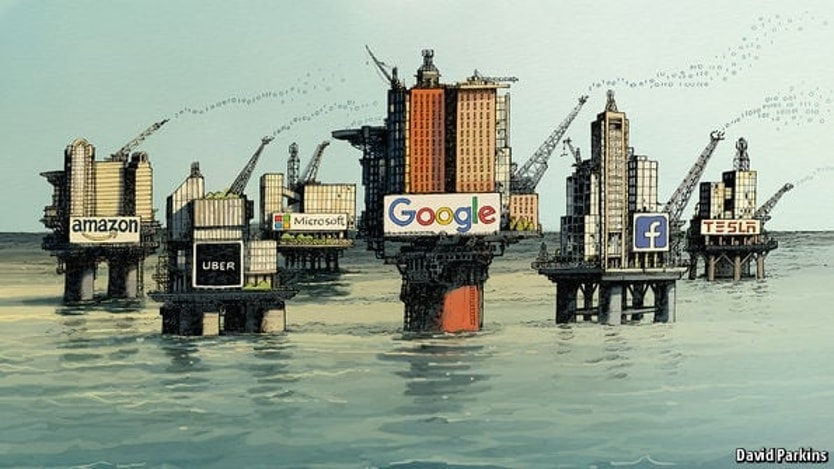
\includegraphics[scale=0.55,height=200pt,width=13cm]{figures/dados1.jpeg}
\caption{Exemplo Referente as Principais Bases de Dados Mundiais.}
\label{fig:my_label8}
\end{figure}


Big data é um termo geral para qualquer coleção de conjuntos de dados tão grandes ou complexos que torna-se difícil processá-los usando técnicas tradicionais de gerenciamento de dados.\vskip0.3cm

Recentemente, em 2013, o termo \textit{Big Data} foi adicionado ao \textit{Oxford English Dictionary} (Dicionário de Oxford para Lígua Inglesa). Em 2014, o Apache Hadoop definiu big data como “conjuntos de dados que não podem ser capturados, gerenciados e processados por computadores em geral dentro de um escopo aceitável”.\vskip0.3cm

O Big Data é caracterizado pelos cinco "Vs":

\begin{itemize}
    \item \textbf{Volume}: Quantidade colossal de dados, geralmente em petabytes (PB) ou exabytes (EB).
    \item \textbf{Variedade}: Diversos tipos de dados, como texto, imagens, vídeos, áudio, dados de sensores, etc
    \item \textbf{Velocidade}: Geração e atualização em tempo real ou quase real, exigindo processamento rápido.
    \item \textbf{Veracidade}: Qualidade e confiabilidade dos dados, essenciais para análises precisas.
    \item \textbf{Valor}: Extração de insights valiosos para embasar decisões estratégicas.
\end{itemize}


A análise de Big Data envolve o uso de técnicas avançadas, como aprendizado de máquina, inteligência artificial, mineração de dados e algoritmos de análise preditiva, para extrair insights significativos dos dados. Esses insights podem ser usados para melhorar a tomada de decisões, prever tendências futuras, otimizar operações e criar novas oportunidades de negócios.


\subsection{Aplicação da Áerea de Trânsito}

O uso de big data na área de trânsito tem o potencial de revolucionar a forma como as cidades lidam com o fluxo de veículos, pedestres e transporte público.\vskip0.3cm 

Aqui estão algumas maneiras pelas quais o big data pode ser aplicado nesse contexto:

\begin{itemize}
    \item \textbf{Gerenciamento de Tráfego em Tempo Real}: Sensores de tráfego, câ\-me\-ras de vigilância e dispositivos GPS podem coletar dados em tempo real sobre o fluxo de veículos e as condições das estradas. Esses dados podem ser analisados para identificar congestionamentos, acidentes ou outras anomalias, permitindo que as autoridades de trânsito tomem medidas rápidas para mitigar problemas.
    \item \textbf{Otimização de Rotas e Planejamento Urbano}: Ao analisar padrões de trá\-fego ao longo do tempo, é possível identificar rotas preferenciais, pontos de congestionamento recorrentes e áreas com necessidade de melhorias na infraestrutura de transporte. Essas informações podem informar o planejamento urbano, ajudando na construção de novas estradas, faixas exclusivas para ônibus, ciclovias e na programação de semáforos.
    \item \textbf{Prevenção de Sinistros}: A análise de dados pode ajudar a identificar padrões de comportamento que aumentam o risco de acidentes, como locais com alta incidência de colisões ou comportamentos de direção agressiva. Com essas informações, as autoridades podem implementar medidas preventivas, como melhor sinalização, instalação de redutores de velocidade e campanhas de conscientização.
    \item \textbf{Melhoria do Transporte Público}: O big data pode ser usado para monitorar a eficiência do transporte público, incluindo a pontualidade dos ônibus e trens, a lotação dos veículos em diferentes horários e rotas, e a satisfação dos passageiros. Essas informações podem ajudar na otimização das rotas, na programação de horários e na alocação de recursos.
\end{itemize}

Em resumo, o uso de big data na área de trânsito pode trazer uma série de benefícios, desde a redução de congestionamentos e tempos de viagem até a melhoria da segurança nas estradas e a eficiência do transporte público. 
%No entanto, é importante garantir que os dados sejam coletados e utilizados de forma ética e respeitando a privacidade dos indivíduos


\subsection{Data Science (Ciência de Dados)}

A Ciência de Dados (Data Science, em inglês) se configura como um campo multidisciplinar que extrai conhecimento e insights valiosos a partir de grandes volumes de dados. Através de técnicas avançadas de estatística, matemática, ciência da computação e aprendizado de máquina.\vskip0.3cm

Você pode pensar na relação entre big data e ciência de dados como sendo a relação entre o petróleo bruto e uma refinaria de petróleo.\vskip0.3cm

A aplicação de Data Science na gestão pública não apenas melhora a eficiência administrativa e operacional, mas também promove uma governança mais transparente, responsável e centrada no cidadão. Ao adotar abordagens baseadas em dados, os governos estão posicionados para enfrentar desafios complexos de forma mais informada e eficaz, promovendo o bem-estar e o desenvolvimento sustentável das comunidades que servem.


\subsection{Machine Learning (Apredizado de Máquina)}

O termo aprendizado de máquina é um método de análise de dados que automatiza a construção de modelos analíticos. É um subcampo ou ramo da inteligência artificial baseado na idéia de que sistemas podem aprender com dados, identificar padrões e tomar decisões com o mínimo de intervenção humana.\vskip0.3cm

Em 1959, Arthur Samuel definiu aprendizado de máquina como o "campo de estudo que dá aos computadores a habilidade de aprender sem serem explicitamente programados.\vskip0.3cm

Um algoritmo de aprendizado é um conjunto de instruções que devem ser compreendidas por um computador para que ele possa aprender com os dados (Mitchell, 1997).\vskip0.3cm

Isso significa que os sistemas criados com Machine Learning podem melhorar seu desempenho ao longo do tempo, à medida que são expostos a mais dados.


\subsubsection{Tipos de Machine Learning}

Didaticamente o Aprendizado de Máquina se divide em:\vskip0.3cm

\subsubsubsection{Aprendizagem Supervisionada}

O algoritmo recebe um conjunto de dados rotulados, onde cada dado tem uma etiqueta que define sua categoria. O objetivo é treinar o algoritmo para identificar a categoria correta de novos dados não rotulados. 
    \\  
    \\
\textbf{Exemplos}: 
\begin{itemize}
\item Classificação de email/spam;
\item Reconhecimento de Imagens;
\item Previsão de Preço de Ações;
\item Previsão de Demandas de Transporte Público;
\end{itemize}

\subsubsubsection{Aprendizagem Não Supervisionada}
O algoritmo recebe um conjunto de dados não rotulados, onde o objetivo é que o mesmo encontre padrões nos dados e os agrupe em categorias significativas. 
\\ 
\\
\textbf{Exemplos}: 
\begin{itemize}
\item Segmentação de Beneficiários para Programas Sociais(CNH Paidegua);
\item Agrupamento de Áreas para Planejamento Urbano;
\item Otimização de Rotas de Coleta de Lixo;
\item Agrupamento de Chamadas de Emergência;
\end{itemize}


\newpage
\subsubsubsection{Aprendizagem Por Reforço}

O algoritmo aprende por tentativa e erro, interagindo com um ambiente. O objetivo é que o mesmo maximize uma recompensa cumulativa ao longo do tempo.
\\
\\
\textbf{Exemplos}:
\begin{itemize}
\item Otimização de Sinais de Trânsito;
\item Alocação de Recurso em Serviços de Emergência;
\item Manutenção Preventiva de Estradas e Pontes;
\item Gestão de Energia em Prédios Públicos;
\end{itemize}

Esses são apenas alguns exemplos de como o Aprendizado de Máquina pode ser aplicado na gestão pública para aumentar a eficiência, reduzir custos e melhorar a qualidade dos serviços prestados aos cidadãos.

\subsection{Storytelling (Contar História com Dados)}

Etimologicamente, a palavra storytelling tem origem na língua inglesa, sendo formada pela junção de duas palavras: story (que significa "história") e telling (que significa "contando" ou "contar"). Portanto, o storytelling é um tipo de comunicação que envolve a narração de histórias (fatos, acontecimentos, fenômenos etc.) com intencionalidades, sejam elas pedagógicas ou informacionais.

%-----------------------------------------------------------------------------------%
\section{Fases ou Etapas de um Levantamento Estatístico}

A pesquisa científica é a aplicação prática de um conjunto de procedimentos objetivos, utilizados por um pesquisador (cientista), para o desenvolvimento de um experimento, a fim de produzir um novo conhecimento, além de integrá-los aqueles pré-existentes. (BARROS et al, 2002). Constituindo-se portanto, em etapas ordenadamente dispostas, de maneira lógica e racional, as quais o pesquisador deverá conhecê-las para aplicá-las convenientemente. (SILVA e MENEZES, 2001). 
\vskip0.3cm


Ao realizar um estudo experimental qualquer ou estatístico completo em determinada população ou em uma parte da mesma (no caso amostra), o trabalho estatístico que se realizará, deverá passar por várias fases onde serão desenvolvidos até se chegar aos resultados finais esperados.\vskip0.3cm

Assim, um levantamento ou trabalho estatístico consiste em um método que pode ser estruturado de tal forma que possibilite seu desenvolvimento nas se\-guintes fases ou etapas: \textbf{Planejamento}, \textbf{Coleta de Dados}, \textbf{Apuração ou Contagem de Dados}, \textbf{Organização, Exposição ou Apresentação de Dados}, \textbf{Análise ou Interpretação de Dados}, \textbf{Relatório Final e Divulgação dos Resultados}.


\subsection{Planejamento}

O planejamento é a etapa inicial do trabalho estatístico, sem duvida representa uma das mais importantes fases do levantamento, nessa etapa procura-se reunir tudo o que existe publicado sobre o fe\-nô\-me\-no a ser estudado, analisando experiências de trabalhos anteriores. Inicialmente, defini-se com clareza o objetivo da pesquisa ou o problema que se pretende pesquisar e, qual é exatamente o objetivo que se deseja alcançar. Porém, não é suficiente saber o que se pretende pesquisar. È também necessário saber onde será realizada a pesquisa: em que \textbf{Local}, com que tipo de \textbf{Pessoas} (ou objetos), em que \textbf{Época} (dias, horários) e assim por diante. Assim, uma vez definido e delimitado o problema, é preciso estar atento a uma série de questões.\vskip0.3cm


O planejamento de uma pesquisa envolve as seguintes etapas:


 \begin{itemize}
\item \textbf{Formulação do Tema e dos Objetivos Gerais e Específicos}: 
A escolha do tema é o primeiro passo para a definição do protocolo de pesquisa. O pesquisador deverá perguntar: "O QUE, DE FATO, QUERO ESTUDAR?". Respondida a pergunta, só então estará apto para pros\-se\-guir com a questão da pesquisa. Nessa fase permite
descobrir as características que se precisa observar ou medir.
Esta parte mostra qual, ou quais são as intenções do pesquisador
em relação ao tema proposto. È aqui onde será informada a proposta
da pesquisa, ou seja, quais os resultados pretendidos ou quais as
contribuições que a pesquisa irá proporcionar ao conhecimento
cinetifico. Estas características determinam as variáveis
estatísticas; Tradicionalmente, os projetos de pesquisa comtemplam
dois tipos de objetivo: o geral e os específicos. Ambos sintetizam
o que o ivestigador pretende esclarecer e devem ser coerentes com
o problema proposto e com a justificativa fornecida. No objetivo
geral, o pesquisador propõe uma síntese dos resultados que
pretende alcançar com a pesquisa; nos objetivos específicos, ele
detalha as propostas desdobradas a partir do objetivo geral. A
princípio, a boa técnica para enunciar o objetivo é começar a sua
redação com um verbo no infinitivo, o qual deverá exprimir uma
ação bem definida, possível de ser executada e de ser mensurada
(FONTELLES, 2009). A escolha do Tema é o primeiro passo para a definição do protocolo de pesquisa. O pesquisador deverá perguntar: "O que, de fato, quero estudar?". Respondida a pergunta, só então estará apto para prosseguir com a questão da pesquisa. Uma vez selecionado o tema, a definição do problema é o passo seguinte e de sua correta formulação, dependerá o sucesso da pesquisa. Embora sempre todos procedimento propostos para a realização da pesquisa deverão ser planejadas no sentido de solucionar o problema proposto. A ordem correta de raciocínio é: "Qual é a questão que necessita de investigação e/ou solução?" 
"O que ela causa?" "O que a minha pesquisa irá contribuir para solucioná-la?".     


\newpage
\item \textbf{Definir o Tipo de Pesquisa}: Para um pesquisador que pretende planejar um experimento, a sequência correta do raciocínio é: primeiro ele deve escolher, entre os diversos tipos de pesquisa, aquele que melhor se enquadra na população a ser estudada e que melhor atende aos seus objetivos. Segundo, definir o melhor delineamento a ser empregado para que os objetivos possam ser alnaçados.O método de levantamento dos dados é um dos mais comuns e mais usuais, seja ele por meio de técnicas de amostragem ou censitário, onde deverá ser definido levando-se em conta as vantagens e desvantagens de cada um deles. Numa pesquisa tipo levantamento, às vezes, é suficiente a pura observação, no entanto, na maioria das vezes, é necessário registrar as características dos elementos da amostra utilizando-se um instrumento de coleta dos dados tais como: questionários, protocolos, roteiros de entrevistas, prontuários médicos, folhas de verificação em fábricas, etc. Nessa etapa deve-se também testar o instrumento de obtenção das informações, evitando no trabalho final a utilização de um instrumento de coleta que não seja eficiente. Com isso, pessoas serão contratadas para a distribuição e aplicação dos questionários ou para elaboração de entrevistas. Aqui reside a maior preocupação dos pesquisadores: Que tipo de pessoa(s) deverá (ão) ser contratada (s)$?$ Que tipo de treinamento essa (s) pessoa (s) deverá (ão) receber$?$
   \item \textbf{População e Amostra}: Nesta etapa deve-se definir o universo ou a população alvo, isto é, o conjunto de elementos que o pesquisador abrange em um determinado estudo ou experimento, para os quais os resultados oriundos da pesquisa sejam válidos. Deve-se também calcular o tamanho mínimo da amostra de forma que a mesma assegure representatividade e um nível de confiança desejável a um nível de erro permitido, ou seja, que as características existentes na população em estudo, estejam contidas na amostra retida.
   \item \textbf{Planejamento da Coleta dos Dados}: Determinar a forma mais e\-co\-nô\-mi\-ca de obtenção das informações da pesquisa.
 \end{itemize}


\subsection{Coleta de Dados}

Esta fase constitui a transposição do projeto do plano abstrato para o campo empírico, representando a \textbf{Execução Operacional do Projeto de Pesquisa}. Se o delineamento inicial e os procedimentos previstos foram planejados de forma consistente, a probabilidade de obter respostas fidedignas e inferências precisas sobre o fenômeno estudado é significativamente elevada (MARCONI et al., 2005).


\newpage
\subsubsection{O Papel Crítico do Estudo Piloto}

Para mitigar vieses e identificar falhas estruturais no planejamento, é imperativa a implementação de um \textbf{Estudo Piloto}. Esta etapa não se resume a uma pré-coleta; trata-se de um procedimento de validação metodológica que fornece subsídios para o cálculo definitivo do tamanho amostral e garante a padronização na aplicação dos instrumentos (FONTELLES, 2009). É no piloto que se testa a clareza da linguagem e a receptividade do respondente, "arredondando" o método antes da mobilização total de recursos.

\subsubsection{Instrumentos e Escalas de Mensuração}

Um dos maiores desafios na coleta de dados em gestão pública é a mensuração de fenômenos que não podem ser observados diretamente, como a \textbf{Maturidade Organizacional}, o \textbf{Clima Ético} ou o \textbf{Bem-estar do Servidor}. Para tanto, o pesquisador utiliza escalas que convertem percepções subjetivas em dados passíveis de análise estatística.\textbf{Principais Escalas Utilizadas em Pesquisas Governamentais:}

\begin{itemize}
\item \textbf{Escala de Likert (Concordância/Satisfação):} A mais difundida mundialmente, mensura a intensidade da opinião (ex: "Discordo Totalmente" a "Concordo Totalmente"). Essencial para avaliar a percepção de usuários sobre serviços públicos.
\item \textbf{Diferencial Semântico:} Utiliza adjetivos bipolares (ex: Eficiente/Ineficiente) para medir a atitude do cidadão frente a uma instituição.
\item \textbf{Escalas Psicométricas (Agressividade, Raiva, Depressão):} Utilizadas em concursos públicos e saúde ocupacional para avaliar o perfil comportamental de agentes de segurança ou servidores em áreas de risco.
\item \textbf{Modelos de Maturidade:} Escalas ordinais que medem o estágio de desenvolvimento de processos em secretarias e órgãos do Estado (Incipiente, Padronizado, Otimizado).
\end{itemize}

\subsubsection{Validade e Fidedignidade}Ao utilizar escalas, a robustez do trabalho estatístico repousa sobre duas propriedades básicas (HAIR et al., 2010):

\begin{enumerate}
\item \textbf{Validade:} O instrumento mede, de fato, o que se propõe a medir? A \textbf{Validade de Construto} é frequentemente verificada via Modelo de \textbf{Análise Fatorial}, garantindo que os itens do questionário capturem a essência do fenômeno.
\item \textbf{Fidedignidade (Reliability):} O procedimento produz resultados consistentes em repetidas tentativas? O indicador padrão-ouro aqui é o Coeficiente \textbf{Alfa de Cronbach} ($\alpha$), que mede a consistência interna das respostas. Valores acima de 0,70 são geralmente aceitos como evidência de um instrumento confiável.
\end{enumerate}

\subsubsection{Tipologia das Questões em Questionários}Didaticamente, as questões podem ser estruturadas conforme a necessidade analítica:

\begin{itemize}
\item \textbf{Questões Fechadas Escalares:} As categorias são itens de escalas (como as de Likert). Permitem análises tanto como variáveis categóricas quanto numéricas (ao atribuir pesos), facilitando o uso de técnicas estatísticas avançadas.
\item \textbf{Questões de Código:} Facilitam a organização de dados estruturados, como o \textbf{Código de Endereçamento Postal (CEP)} ou o \textbf{Número de Identificação Social (NIS)}, cruciais para a geolocalização de políticas públicas.
\item \textbf{Questões Abertas Textuais:} Fundamentais para a análise qualitativa ou para técnicas de \textit{Text Mining} e Análise de Sentimento, permitindo captar a "voz" do cidadão de forma livre.
\end{itemize}

Para facilitar o processo de planejamento da coleta, a Tabela \ref{tab:escalas_famosas} apresenta modelos de escalas consolidados na literatura científica e amplamente aplicáveis ao diagnóstico organizacional e social na gestão pública.

\begin{table}[H]
\centering
\caption{Principais Escalas de Mensuração para Gestão e Pesquisa Social}
\label{tab:escalas_famosas}
\small
\begin{tabular}{l|p{5cm}|p{4cm}}
\hline
\textbf{Escala} & \textbf{Construto} & \textbf{Aplicação} \\ \hline
\textbf{Likert} & Intensidade de concordância ou satisfação. & Avaliação de serviços e clima organizacional. \\  \hline
\textbf{Guttman} & Atitudes acumulativas e hierárquicas. & Medir o grau de aceitação de políticas públicas progressivas. \\  \hline
\textbf{Diferencial Semântico} & Atitude emocional ou cognitiva perante conceitos. & Imagem institucional de órgãos perante a população. \\  \hline
\textbf{PANAS} & Afetos Positivos e Negativos. & Monitoramento da saúde mental e estresse de agentes de segurança. \\  \hline
\textbf{SERVQUAL} & Qualidade percebida versus expectativa. & Auditoria de qualidade em serviços de atendimento ao cidadão. \\  \hline
\textbf{Resiliência} & Capacidade de adaptação a crises e mudanças. & Avaliação de lideranças e equipes em contextos de emergência. \\  \hline
\end{tabular}
\end{table}

%------------------------------------------------------------------------------%
\subsection{Apuração, Crítica e Processamento de Dados}

Após o encerramento da coleta, o pesquisador defronta-se com um volume bruto de informações numéricas e textuais que, isoladamente, não constituem conhecimento. Esta fase compreende a transição da coleta para a análise, envolvendo a crítica, a tabulação e a organização sistemática dos dados para garantir a precisão dos cálculos estatísticos subsequentes (SILVA; MENEZES, 2001).

\subsubsection{Crítica e Saneamento (Data Cleaning)}

Antes de qualquer procedimento analítico, é imperativo realizar a Crítica de Dados. Este processo consiste em examinar o material coletado para identificar e corrigir inconsistências, omissões ou erros que possam enviesar os resultados. Na gestão pública, onde as decisões impactam orçamentos vultosos, o saneamento de dados é uma salvaguarda ética. \vskip0.3cm

\textbf{Procedimentos de Saneamento:}

\begin{itemize}
\item \textbf{Tratamento de Dados Omissos (\textit{Missing Data}):} Identificar se a ausência de resposta segue um padrão (ex: cidadãos de baixa renda evitam responder sobre impostos). O gestor deve decidir entre a exclusão do registro ou o uso de técnicas de imputação.
\item \textbf{Identificação de \textit{Outliers} (Valores Atípicos):} Detectar dados que fogem drasticamente da realidade (ex: uma idade registrada como 150 anos). Deve-se verificar se é um erro de digitação ou um fenômeno raro que merece estudo à parte.
\item \textbf{Padronização de Variáveis:} Ajustar unidades de medida (ex: converter tudo para metros ou quilômetros) e corrigir divergências de digitação (ex: "DETRAN", "detran", "DeTran") para garantir que o software contabilize as categorias corretamente.
\end{itemize}

\subsubsection{Tecnologias de Processamento}

A apuração pode ser manual em estudos de pequena escala, mas a complexidade da administração pública contemporânea exige o uso de recursos computacionais. A escolha do software deve considerar não apenas a capacidade de processamento, mas a Reprodutibilidade das Análises.

\begin{itemize}
\item \textbf{Softwares Proprietários:} \textbf{SPSS}, \textbf{SAS}, \textbf{Stata} e \textbf{Minitab} são amplamente utilizados pela interface amigável e suporte técnico.
\item \textbf{Ecossistema de Código Aberto (Open Source):} O uso de linguagens como \textbf{R} e \textbf{Python} tem crescido exponencialmente na gestão pública. Elas permitem a criação de \textit{scripts} que podem ser auditados por qualquer cidadão, atendendo aos princípios da Lei de Acesso à Informação e garantindo que a análise possa ser replicada com os mesmos resultados.
\end{itemize}

\subsubsection{Ciência de Dados na Gestão Pública}

Com a automação, a apuração deixou de ser um simples resumo de contagem para se tornar uma base segura para a elaboração de índices complexos, painéis de monitoramento (\textit{dashboards}) e modelos preditivos. A segurança no manejo das informações nesta fase é o que permite ao gestor afirmar que a sua decisão não é baseada em uma percepção isolada, mas em um corpo de dados íntegro e verificado.


\begin{tcolorbox}[colback=green!5,colframe=green!40!black,title= Dica Técnica: Reprodutibilidade e Transparência]
Na gestão pública moderna, a apuração de dados deve ser \textbf{reprodutível}. Recomenda-se que o pesquisador armazene o banco de dados original (bruto) e registre em um log de alterações (ou script de programação) cada limpeza ou exclusão feita durante a fase de crítica. Isso garante a transparência do processo e permite que auditorias comprovem a integridade dos resultados finais.
\end{tcolorbox}


%------------------------------------------------------------------------------%


%------------------------------------------------------------------------------%
\subsection{Organização, Exposição dos Dados}

A apresentação de dados é a interface entre o rigor estatístico e a tomada de decisão. Uma vez apurados, os dados devem ser expostos em tabelas ou gráficos, respeitando a premissa de que a forma deve sempre servir à clareza da mensagem.

\subsubsection{O Rigor Tabular (Normas IBGE/ABNT)}

A forma tabular é o modo formal de exposição dos resultados, permitindo o cruzamento de variáveis e a consulta precisa de valores. Para que uma tabela seja tecnicamente correta na administração pública brasileira, ela deve seguir as Normas de Apresentação Tabular do IBGE e ABNT.

%\begin{itemize}
%\item Título: Deve responder "O quê?", "Onde?" e "Quando?", "Porquê?".
%\item Cabeçalho: Identifica o conteúdo das colunas.
%\item Corpo: O conjunto de dados propriamente dito.
%\item Fonte: Essencial para a transparência e rastreabilidade da informação.
%\end{itemize}


\subsubsection{Análise, Interpretação e a Incerteza Científica}

A análise constitui o ápice do levantamento estatístico. É nesta etapa que técnicas consolidadas como estatísticas descritivas, testes de hipóteses e modelos explicativos são aplicadas para transformar dados em conclusões resolutivas. \vskip0.3cm

O grande desafio reside na Inferência Estatística: o processo de tirar conclusões sobre uma população a partir de uma amostra. Este movimento envolve sempre um grau de incerteza, quantificado pelo erro amostral e pelo nível de confiança. Um bom relatório deve ser honesto sobre essas limitações, evitando generalizações temerárias que possam comprometer políticas públicas.


\newpage
\subsubsection{Relatório Final}

O relatório final é o documento que consagra a pesquisa. Seja um relatório executivo, uma dissertação ou um artigo científico, a redação deve possuir o que chamamos de beleza técnica: clareza nas ideias, precisão nas informações e uma estrutura que respeite as normas da ABNT ou de instituições específicas. \vskip0.3cm

A escrita científica é um exercício de honestidade intelectual. O texto deve ser agradável, mas nunca à custa da precisão. Conclusões devem ser justificadas estritamente pelos dados apresentados, e a metodologia deve ser descrita com detalhes suficientes para permitir a reprodutibilidade.


\subsubsection{Diretrizes para Avaliação Crítica}

Para garantir que o método estatístico não seja enviesado, adaptamos as diretrizes de Triola (2005) para uma auditoria crítica de levantamentos:


\begin{itemize}
\item \textbf{Objetivo e População}: Estão claramente definidos ou o estudo é vago?;
\item Fonte e Tendenciosidade: Quem financiou ou coletou os dados? Há conflitos de interesse?;
\item Método de Amostragem: A amostra é representativa ou foi selecionada por conveniência?;
\item Definição de Variáveis: As variáveis medem realmente o que se pretendia (Validade)?;
\item Confundimento: Existem variáveis ocultas que podem estar distorcendo a relação entre causa e efeito?;
\item Fraseado das Questões: As perguntas do questionário induzem a uma resposta específica?;
\item Integridade Gráfica: Os gráficos possuem escalas honestas ou estão visualmente distorcidos para exagerar resultados?;
\item Significado Prático: Além da significância estatística, o resultado tem relevância real para a vida do cidadão e para o erário?
\end{itemize}

\vskip0.3cm

\begin{tcolorbox}[colback=green!5,colframe=green!40!black,title=Conclusão: Do Dado à Decisão]
A estatística na gestão pública não termina no cálculo de uma média ou na plotagem de um gráfico. Ela se realiza quando o relatório final fornece a evidência necessária para que o gestor possa alocar recursos com justiça, eficiência e transparência. Assim, a estatística governamental é o bem-estar social fundamentado na verdade dos dados.
\end{tcolorbox}